\part{Filtro con GIC}
\section{Introducción}
Un circuito GIC(generalized impedance converter) es un circuito RC activo diseñado para simular componentes que varían su comportamiento dependiendo de la frecuencia para usar, por ejemplo, en el diseño de filtros activos como es el caso del presente trabajo.
Se presentará a continuación el análisis y la implementación de un filtro pasa banda activo, implementado un GIC simulando una inductancia. Se detallarán los cálculos que nos permiten obtener su trasferencia, así como también se desarrollará el criterio para elegir los componentes que lo conforman, en función de una serie de condiciones preestablecidas.

\section{Transferencia del circuito}
\subsection{Impedancia equivalente y transferencia del GIC}

La impedancia equivalente que se presenta entre los terminales del circuito esta descripta, en función de las impedancias que lo compongan, por la expresion \ref{exp:impedancia_gic}

\begin{equation}
Z = \frac{Z_1Z_3Z_5}{Z_2Z_4}
\label{exp:impedancia_gic}
\end{equation}



\begin{figure}[h]
\centering
\begin{circuitikz}[scale=0.65, transform shape]

	\node [label=above:$V$](VGIC) at (0,0){};
	\node [below=1cm of VGIC](n1){};
	\node [below=1cm of n1](n2){};
	\node [below=1cm of n2](n3){};
	\node [below=1cm of n3](n4){};
	\node [below=1cm of n4](n5){};
	\node [below=1cm of n5](n6){};
	\node [below=1cm of n6](n7){};
	\node [below=1cm of n7](n8){};
	\node [below=1cm of n8](n9){};
	\node [below=1cm of n9](n10){};
	\node [below=1cm of n10](GND){};
	

	
	\node (Vp1) at ($(VGIC)!0.5!(n1)$){};
	\node (Vo2) at ($(n2)!0.5!(n3)$){};
	\node (Vn) 	at ($(n4)!0.5!(n5)$){};
	\node (Vo1) at ($(n6)!0.5!(n7)$){};
	\node (Vp2) at ($(n8)!0.5!(n9)$){};
	
	\node [right=1cm of Vp1](n11){};
	\node [right=1cm of Vn](n12){};
	\node [left=1cm of Vn](n13){};
	\node [left=1cm of Vp2](n14){};
		
	\node [right=2.5cm of Vo2](nop1){};
	\node [left=2.5cm of Vo1](nop2){};

	\draw (VGIC) to[short, o-] (n1);
	\draw (n1) to[generic=$Z_1$,-] (n2);
	\draw (n2) to[short] (n3);
	\draw (n3) to[generic=$Z_2$,-] (n4);
	\draw (n4) to[short] (n5);
	\draw (n5) to[generic=$Z_3$,-] (n6);
	\draw (n6) to[short] (n7);
	\draw (n7) to[generic=$Z_4$,-] (n8);
	\draw (n8) to[short] (n9);
	\draw (n9) to[generic=$Z_5$,-] (n10);
	\draw (n10) to[short, -] (GND) node[ground]{};
	
	\draw (nop1) node[op amp,yscale=-1](amp1){};
	\draw (nop2) node[op amp,rotate=180,yscale=-1](amp2){};
	
	\draw (Vp1) to[short,*-] (n11);
	\draw (n11) to[short,-] (n11 |- amp1.+) to[short,-] (amp1.+);
	
	\draw (Vn) to[short,*-] (n12);
	\draw (n12) to[short,-] (n12 |- amp1.-) to [short,-] (amp1.-);	
	
	\draw (amp1.out) to[short,-] ++(1,0) coordinate (right_amp1);
	\draw (right_amp1) to[short] (right_amp1 |- Vo1) to[short,-*] (Vo1);
	\draw (right_amp1) to[short, -o] ++(1,0) node[label=right:$V_{out}$](){};
	
	\draw (Vn) to[short,*-] (n13);
	\draw (n13) to[short,-] (n13 |- amp2.-) to [short,-] (amp2.-);	
	
	\draw (Vp2) to[short,*-] (n14);
	\draw (n14) to[short,-] (n14 |- amp2.+) to[short,-] (amp2.+);
	
	\draw (amp2.out) to[short,-] ++(-1,0) coordinate (right_amp2);
	\draw (right_amp2) to[short] (right_amp2 |- Vo2) to[short,-*] (Vo2);

\end{circuitikz}
\caption{Circuito GIC genérico}
\label{fig:1_gic_generico}
\end{figure}

La Figura \ref{fig:1_gic_aislado} muestra el circuito GIC que se utilizó para simular una inductancia. Al evaluar los valores de los componentes del circuito de la Figura \ref{fig:1_gic_aislado} en la Expresión \ref{exp:impedancia_gic}, obtenemos la impedancia equivalente Z, y de esa forma podemos determinar el comportamiento del circuito.

\[
Z = \frac{R_1R_3R_8}{R_4 \frac{1}{j\omega C_2}} = \frac{R_1R_3R_8C_2j\omega}{R_4}
\]

Si llamamos

\[
L_{GIC} = \frac{R_1R_3R_8C_2}{R_4}
\]

Podemos ver que la impedancia equivalente del circuito se comporta como una inductancia de valor $L_{GIC}$, y podemos definir

\[
Z = L_{GIC}j\omega
\]


\begin{figure}[h]
\centering
\begin{circuitikz}[scale = 0.65, transform shape]

	\node [label=above:$v_{GIC}$](VGIC) at (0,0){};
	\node [below=1cm of VGIC](n1){};
	\node [below=1cm of n1](n2){};
	\node [below=1cm of n2](n3){};
	\node [below=1cm of n3](n4){};
	\node [below=1cm of n4](n5){};
	\node [below=1cm of n5](n6){};
	\node [below=1cm of n6](n7){};
	\node [below=1cm of n7](n8){};
	\node [below=1cm of n8](n9){};
	\node [below=1cm of n9](n10){};
	\node [below=1cm of n10](GND){};
	

	
	\node (Vp1) at ($(VGIC)!0.5!(n1)$){};
	\node (Vo2) at ($(n2)!0.5!(n3)$){};
	\node (Vn) 	at ($(n4)!0.5!(n5)$){};
	\node (Vo1) at ($(n6)!0.5!(n7)$){};
	\node (Vp2) at ($(n8)!0.5!(n9)$){};
	
	\node [right=1cm of Vp1](n11){};
	\node [right=1cm of Vn](n12){};
	\node [left=1cm of Vn](n13){};
	\node [left=1cm of Vp2](n14){};
		
	\node [right=2.5cm of Vo2](nop1){};
	\node [left=2.5cm of Vo1](nop2){};

	\draw (VGIC) to[short, o-] (n1);
	\draw (n1) to[R=$R_1$,-] (n2);
	\draw (n2) to[short] (n3);
	\draw (n3) to[C=$C_2$,-] (n4);
	\draw (n4) to[short] (n5);
	\draw (n5) to[R=$R_3$,-] (n6);
	\draw (n6) to[short] (n7);
	\draw (n7) to[R=$R_5$,-] (n8);
	\draw (n8) to[short] (n9);
	\draw (n9) to[R=$R_8$,-] (n10);
	\draw (n10) to[short, -] (GND) node[ground]{};
	
	\draw (nop1) node[op amp,yscale=-1](amp1){};
	\draw (nop2) node[op amp,rotate=180,yscale=-1](amp2){};
	
	\draw (Vp1) to[short,*-] (n11);
	\draw (n11) to[short,-] (n11 |- amp1.+) to[short,-] (amp1.+);
	
	\draw (Vn) to[short,*-] (n12);
	\draw (n12) to[short,-] (n12 |- amp1.-) to [short,-] (amp1.-);	
	
	\draw (amp1.out) to[short,-] ++(1,0) coordinate (right_amp1);
	\draw (right_amp1) to[short] (right_amp1 |- Vo1) to[short,-*] (Vo1);
	\draw (right_amp1) to[short, -o] ++(1,0) node[label=right:$V_{out}$](){};
	
	\draw (Vn) to[short,*-] (n13);
	\draw (n13) to[short,-] (n13 |- amp2.-) to [short,-] (amp2.-);	
	
	\draw (Vp2) to[short,*-] (n14);
	\draw (n14) to[short,-] (n14 |- amp2.+) to[short,-] (amp2.+);
	
	\draw (amp2.out) to[short,-] ++(-1,0) coordinate (right_amp2);
	\draw (right_amp2) to[short] (right_amp2 |- Vo2) to[short,-*] (Vo2);

\end{circuitikz}
\caption{Circuito GIC utilizado}
\label{fig:1_gic_aislado}
\end{figure}

La transferencia del circuito de la Figura \ref{fig:1_gic_aislado} está dada por la Expresión \ref{exp:transferencia_GIC}

\begin{equation}
\frac{V_{out}}{V_{GIC}} = \left(1 + \frac{R_4}{R_8}\right)
\label{exp:transferencia_GIC}
\end{equation}

\subsection{Transferencia del filtro}\label{section_transf_filtro}
La Figura \ref{circuito_induct} muestra el filtro a implementar. Como se explicó anteriormente, el GIC se comporta como una inductancia de valor $L_{GIC}$. De esta forma, se puede hallar la transferencia desde $v_{in}$ hacia el GIC (representado por el inductor en la Figura ), y luego hallar la transferencia desde el GIC hacia $V_{out}$

\begin{figure}[h]
\centering
\begin{circuitikz}
\node [label=left:$V_{in}$](Vin) at (0,0){};
\node [right=3cm of Vin](Vc){};
\node [right=0.5cm of Vc,label=above:$V_{GIC}$](VGIC){};
\node [right=0.5cm of VGIC](VL){};

\draw (Vin) to[R=$R_6$,o-] (Vc);
\draw (Vc) to[C=$C_6$] ++(0,-2) node[ground]{};
\draw (Vc) to[short, -o] (VGIC);
\draw (VGIC) to[short,o-] (VL);
\draw (VL) to[L=$L_{GIC}$] ++(0,-2) node[ground]{};
\end{circuitikz}
\caption{Filtro con inductancia equivalente}
\label{circuito_induct}
\end{figure}

La transferencia de $V_{in}$ a $V_{GIC}$ esta dada por la Expresión \ref{exp:transf_vin_vgic}.

\begin{equation}
\frac{V_{GIC}}{V_{in}} = \frac{\frac{1}{R_6C_6}\$}{\$^2 + \frac{1}{R_6C_6}\$ + \frac{1}{L_{GIC}C_6}}
\label{exp:transf_vin_vgic}
\end{equation}

Combinando las expresiones \ref{exp:transferencia_GIC} y \ref{exp:transf_vin_vgic}, se obtiene la Expresión  , la cual expresa la tansferencia total del filtro.

\begin{figure}[h]
\centering
\begin{circuitikz}[scale = 0.7, transform shape]

	\node [label=above:$v_{GIC}$](VGIC) at (0,0){};
	\node [below=2cm of VGIC](n1){};
	\node [below=1cm of n1](n2){};
	\node [below=1cm of n2](n3){};
	\node [below=1cm of n3](n4){};
	\node [below=1cm of n4](n5){};
	\node [below=1cm of n5](n6){};
	\node [below=1cm of n6](n7){};
	\node [below=1cm of n7](n8){};
	\node [below=1cm of n8](n9){};
	\node [below=1cm of n9](n10){};
	\node [below=1cm of n10](GND){};
	
	\node [left=2cm of VGIC](Vc){};
	\node [left=4cm of Vc, label=left:$v_{in}$](Vin){};
	
	\draw (Vin) to[R=$R_6$,o-] (Vc);
	\draw (Vc) to[C=$C_6$,*-] ++(0,-2) node[ground]{};
	\draw (Vc) to[short, o-o] (VGIC);

	
	\node (Vp1) at ($(VGIC)!0.5!(n1)$){};
	\node (Vo2) at ($(n2)!0.5!(n3)$){};
	\node (Vn) 	at ($(n4)!0.5!(n5)$){};
	\node (Vo1) at ($(n6)!0.5!(n7)$){};
	\node (Vp2) at ($(n8)!0.5!(n9)$){};
	
	\node [right=1cm of Vp1](n11){};
	\node [right=1cm of Vn](n12){};
	\node [left=1cm of Vn](n13){};
	\node [left=1cm of Vp2](n14){};
		
	\node [right=2.5cm of Vo2](nop1){};
	\node [left=2.5cm of Vo1](nop2){};

	\draw (VGIC) to[short, o-] (n1);
	\draw (n1) to[R=$R_1$,-] (n2);
	\draw (n2) to[short] (n3);
	\draw (n3) to[C=$C_2$,-] (n4);
	\draw (n4) to[short] (n5);
	\draw (n5) to[R=$R_3$,-] (n6);
	\draw (n6) to[short] (n7);
	\draw (n7) to[R=$R_5$,-] (n8);
	\draw (n8) to[short] (n9);
	\draw (n9) to[R=$R_8$,-] (n10);
	\draw (n10) to[short, -] (GND) node[ground]{};
	
	\draw (nop1) node[op amp,yscale=-1](amp1){};
	\draw (nop2) node[op amp,rotate=180,yscale=-1](amp2){};
	
	\draw (Vp1) to[short,*-] (n11);
	\draw (n11) to[short,-] (n11 |- amp1.+) to[short,-] (amp1.+);
	
	\draw (Vn) to[short,*-] (n12);
	\draw (n12) to[short,-] (n12 |- amp1.-) to [short,-] (amp1.-);	
	
	\draw (amp1.out) to[short,-] ++(1,0) coordinate (right_amp1);
	\draw (right_amp1) to[short] (right_amp1 |- Vo1) to[short,-*] (Vo1);
	\draw (right_amp1) to[short, -o] ++(1,0) node[label=right:$V_{out}$](){};
	
	\draw (Vn) to[short,*-] (n13);
	\draw (n13) to[short,-] (n13 |- amp2.-) to [short,-] (amp2.-);	
	
	\draw (Vp2) to[short,*-] (n14);
	\draw (n14) to[short,-] (n14 |- amp2.+) to[short,-] (amp2.+);
	
	\draw (amp2.out) to[short,-] ++(-1,0) coordinate (right_amp2);
	\draw (right_amp2) to[short] (right_amp2 |- Vo2) to[short,-*] (Vo2);

\end{circuitikz}
\caption{Circuito implementado completo}
\label{fig:6_circuito_completo}
\end{figure}

\begin{equation}
\frac{V_{out}}{V_{in}} = \left(1+\frac{R_4}{R_8}\right) \frac{\frac{1}{R_6C_6}\$}{\$^2 + \frac{1}{R_6C_6}\$ + \frac{1}{L_{GIC}C_6}}
\label{1_transfer_completa}
\end{equation}

La transferencia hallada se corresponde con la transferencia de un filtro pasa banda de segundo orden, cuya expresión general está dada por la Expresión \ref{1_transf_generic}. De esta forma, comparando las expresiones podemos determinar las magnitudes relevantes de la misma.

\begin{equation}
H(\$) = K\frac{\frac{\omega_0}{Q}\$}{\$^2 + \frac{\omega_0}{Q}\$ + \omega_0^2}
\label{1_transf_generic}
\end{equation}

\[
\omega_0 = \sqrt{\frac{1}{L_{GIC}C_6}}
\]

\[
Q = R_6 \sqrt{\frac{C_6}{L_{GIC}}}
\]

Se establecen las siguientes relaciones entre los componentes del circuito, de forma que se pueda expresar la transferencia del filtro en función de los componentes que lo conforman, a la que llamaremos a partir de ahora $H(\$)$

\[
R_1 = R_3 = R_4 = R_8 = R
\]

\[
R_6 = QR
\]

\[
C_2 = C_6 = C
\]

\[
H(\$) = 2 \frac{\frac{1}{R_6C}\$}{\$^2 + \frac{1}{R_6C}\$ + \frac{1}{(RC)^2}}
\]

\subsubsection{Función de $R_8$}

Cuando $R_8$ tiende a infinito, el circuito GIC queda flotante, es decir sin conexión a tierra, y de esta forma la impedancia es infinita, y se comporta como un circuito abierto. De esta forma, la transferencia total del filtro se reduce a la siguiente expresión

\[
H(\$) = \frac{1}{1 + \frac{\$}{\omega_c}}
\]

La cuál caracteriza un filtro pasa bajos con frecuencia de corte $\omega_c = \frac{1}{R_6C_6}$


\subsection{Comportamiento de $R_6$}\label{1_seccion_r6}

Si establecemos las siguientes relaciones entre los componentes del circuito, podemos analizar el comportamiento del mismo en función de la relación entre los valores de tres parámetros, $R$, $C$ y $Q$


\[R_1=R_3=R_4=R_8 = R \]
\[R_6 = QR\] 
\[C_2=C_6=C\]

Al desarrollar la expresión de la transferencia remplazando por los valores indicados, se obtiene la siguiente expresión, expresada en función de la frecuencia central del filtro $\omega_0 = \frac{1}{RC}$

\[
H(\$) = 2 \frac{\frac{\omega_0}{Q}\$}{\$^2 + \frac{\omega_0}{Q}\$ + \omega_0^2}
\]

Y de esta forma se puede establecer una caracterización de los polos de la función transferencia en función de la relación entre $R_6$ y $R$, establecida por $Q$. Sean $\$_{1,2}$ los polos del sistema

\begin{equation}
\$_{1,2} = \frac{\omega_0}{2Q}\left(-1 \pm \sqrt{1-4Q^2}\right)
\label{exp_1_polos}
\end{equation}

De la Expresión \ref{exp_1_polos} se determinan los tres casos particulares: dos polos reales distintos, dos polos complejos conjugados, un polo doble real. Las condiciones son, respectivamente:

\begin{subequations}
\begin{align*}
  Q &< 1/2, & R_6 &< \frac{1}{2} R, &\text{2 polos reales} \\
  Q &> 1/2, & R_6 &> \frac{1}{2} R, &\text{2 polos complejos conjugados} \\
  Q &= 1/2, & R_6 &= \frac{1}{2} R, &\text{1 polo real doble}
\end{align*}
\end{subequations}

Las figuras \ref{1_polos_reales}, \ref{1_polos_complejos} y \ref{1_polo_doble} muestran la distribución de los polos del circuito para los tres casos mencionados.

\begin{figure}[ht]
\centering
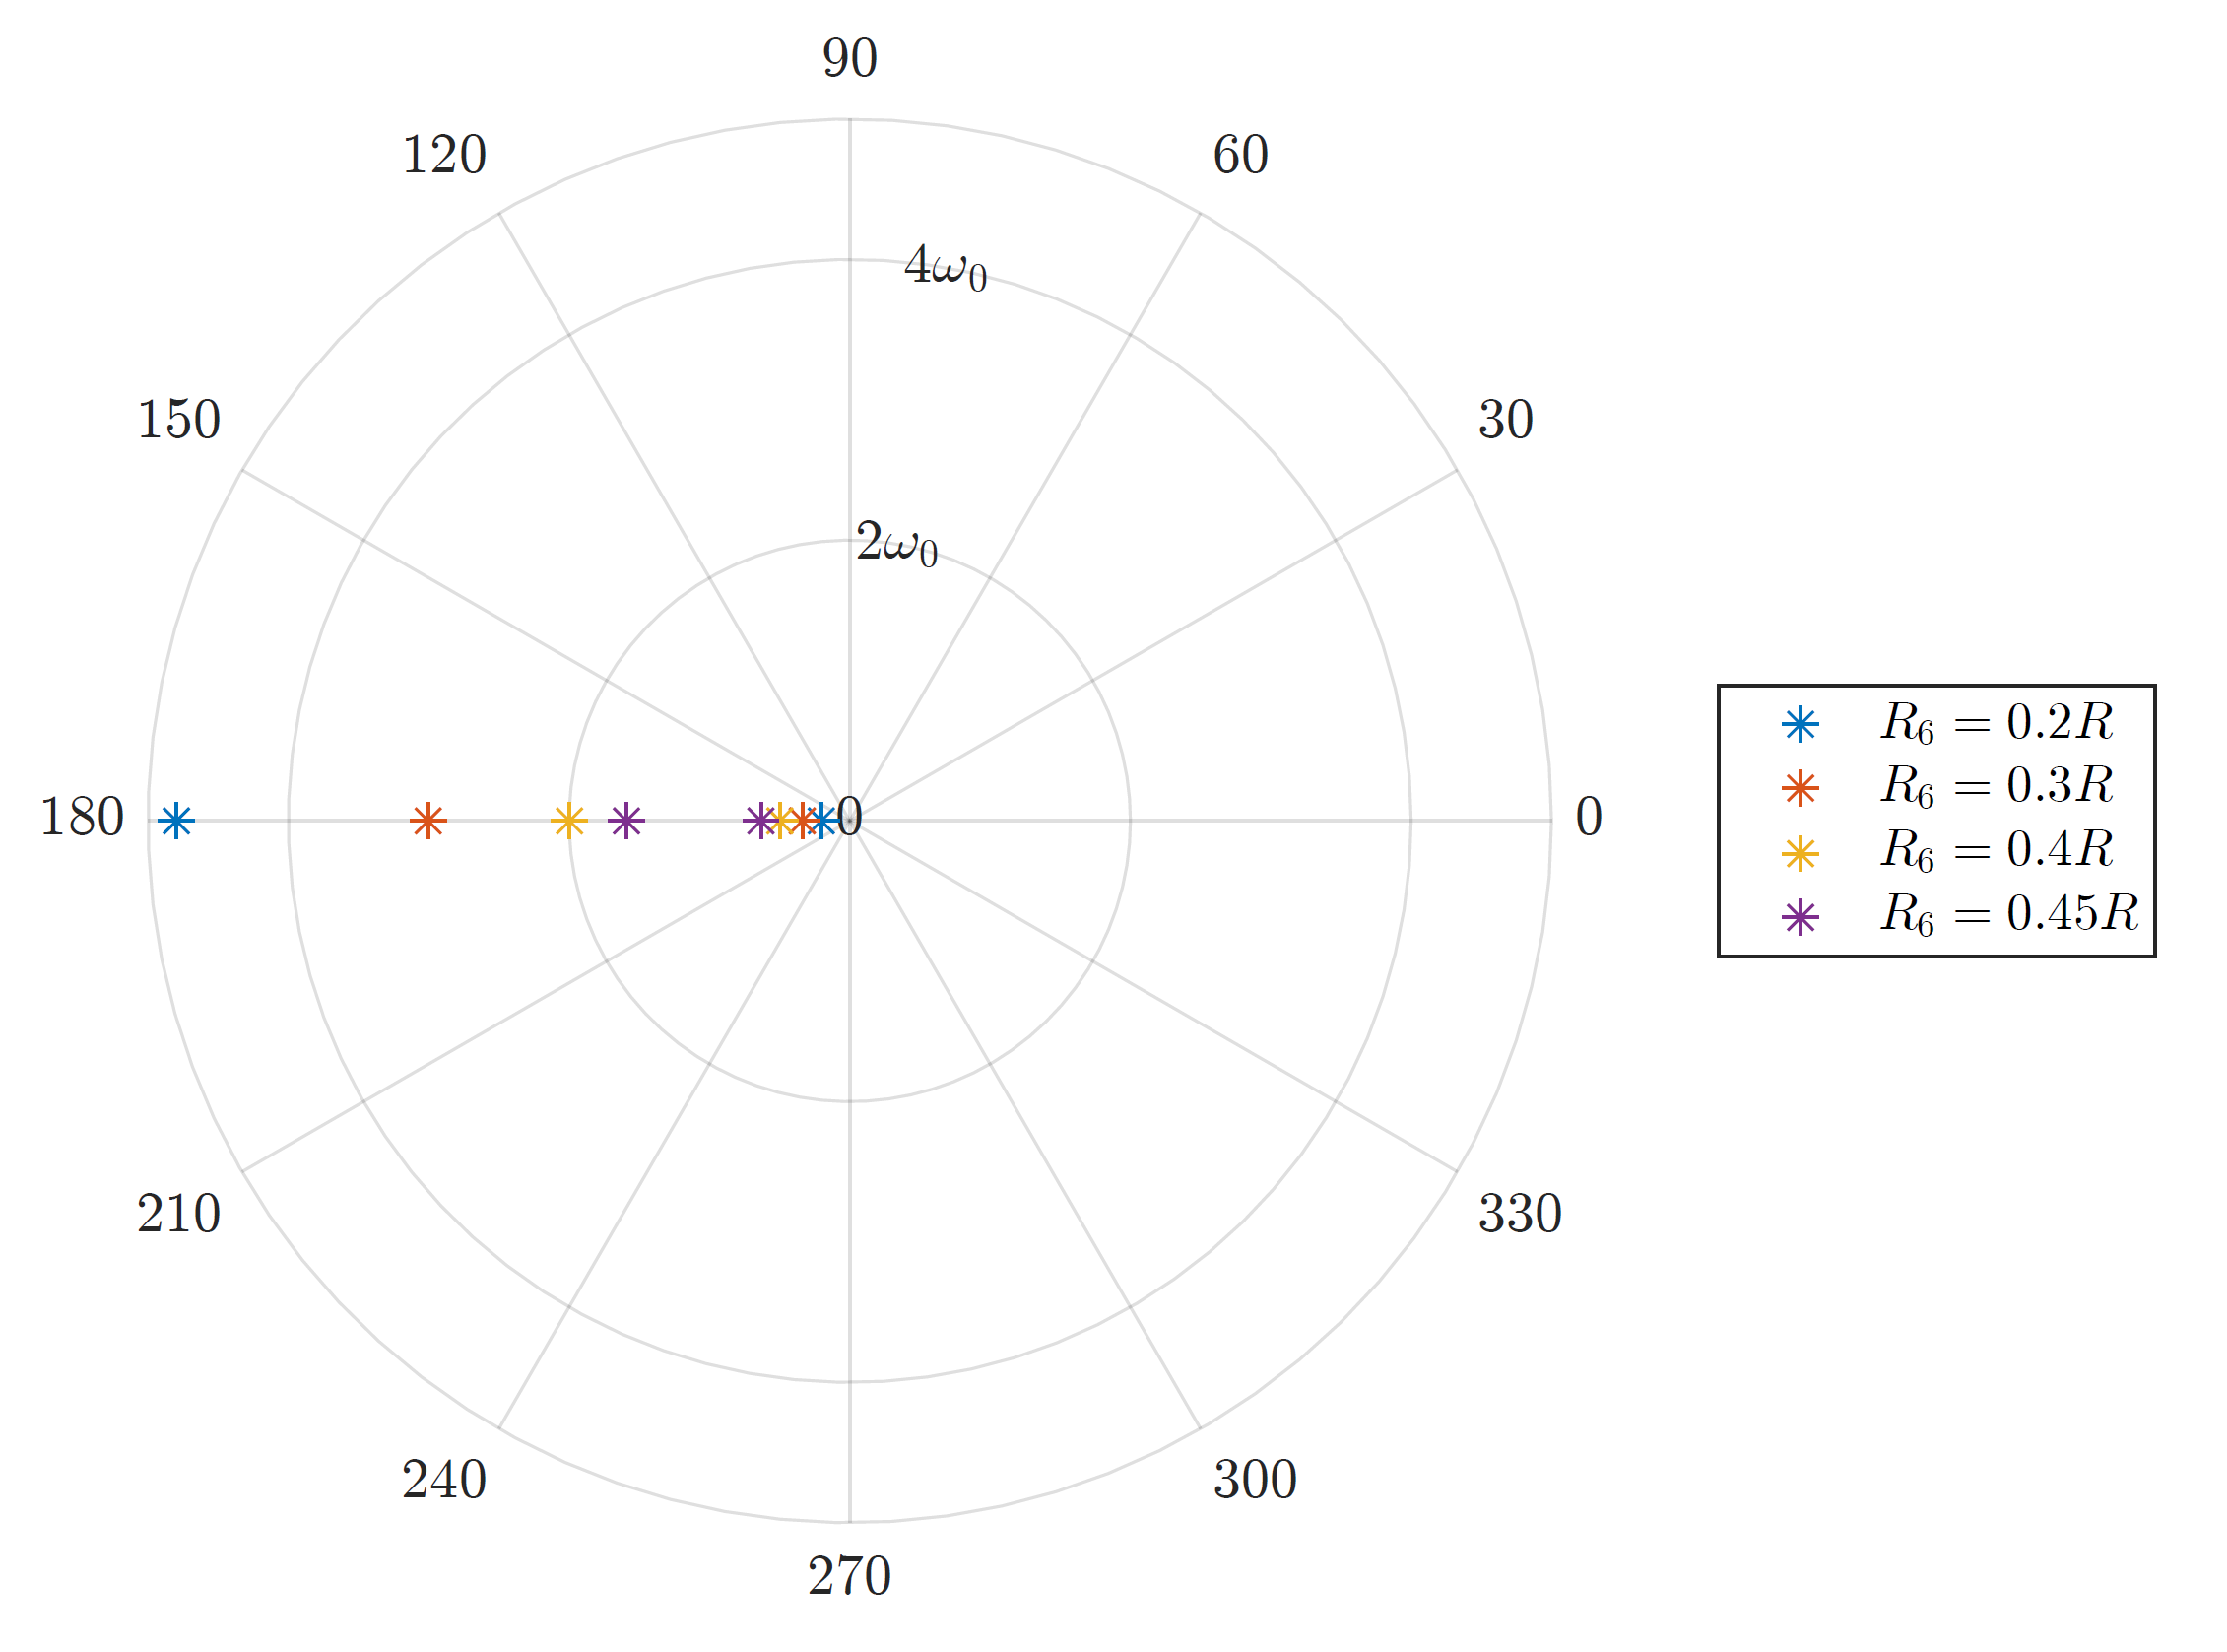
\includegraphics[scale=0.5]{../parte1/informe/resources/1_polos_reales}
\caption{Distribución de polos. Dos polos reales}
\label{1_polos_reales}
\end{figure}

\begin{figure}[ht]
\centering
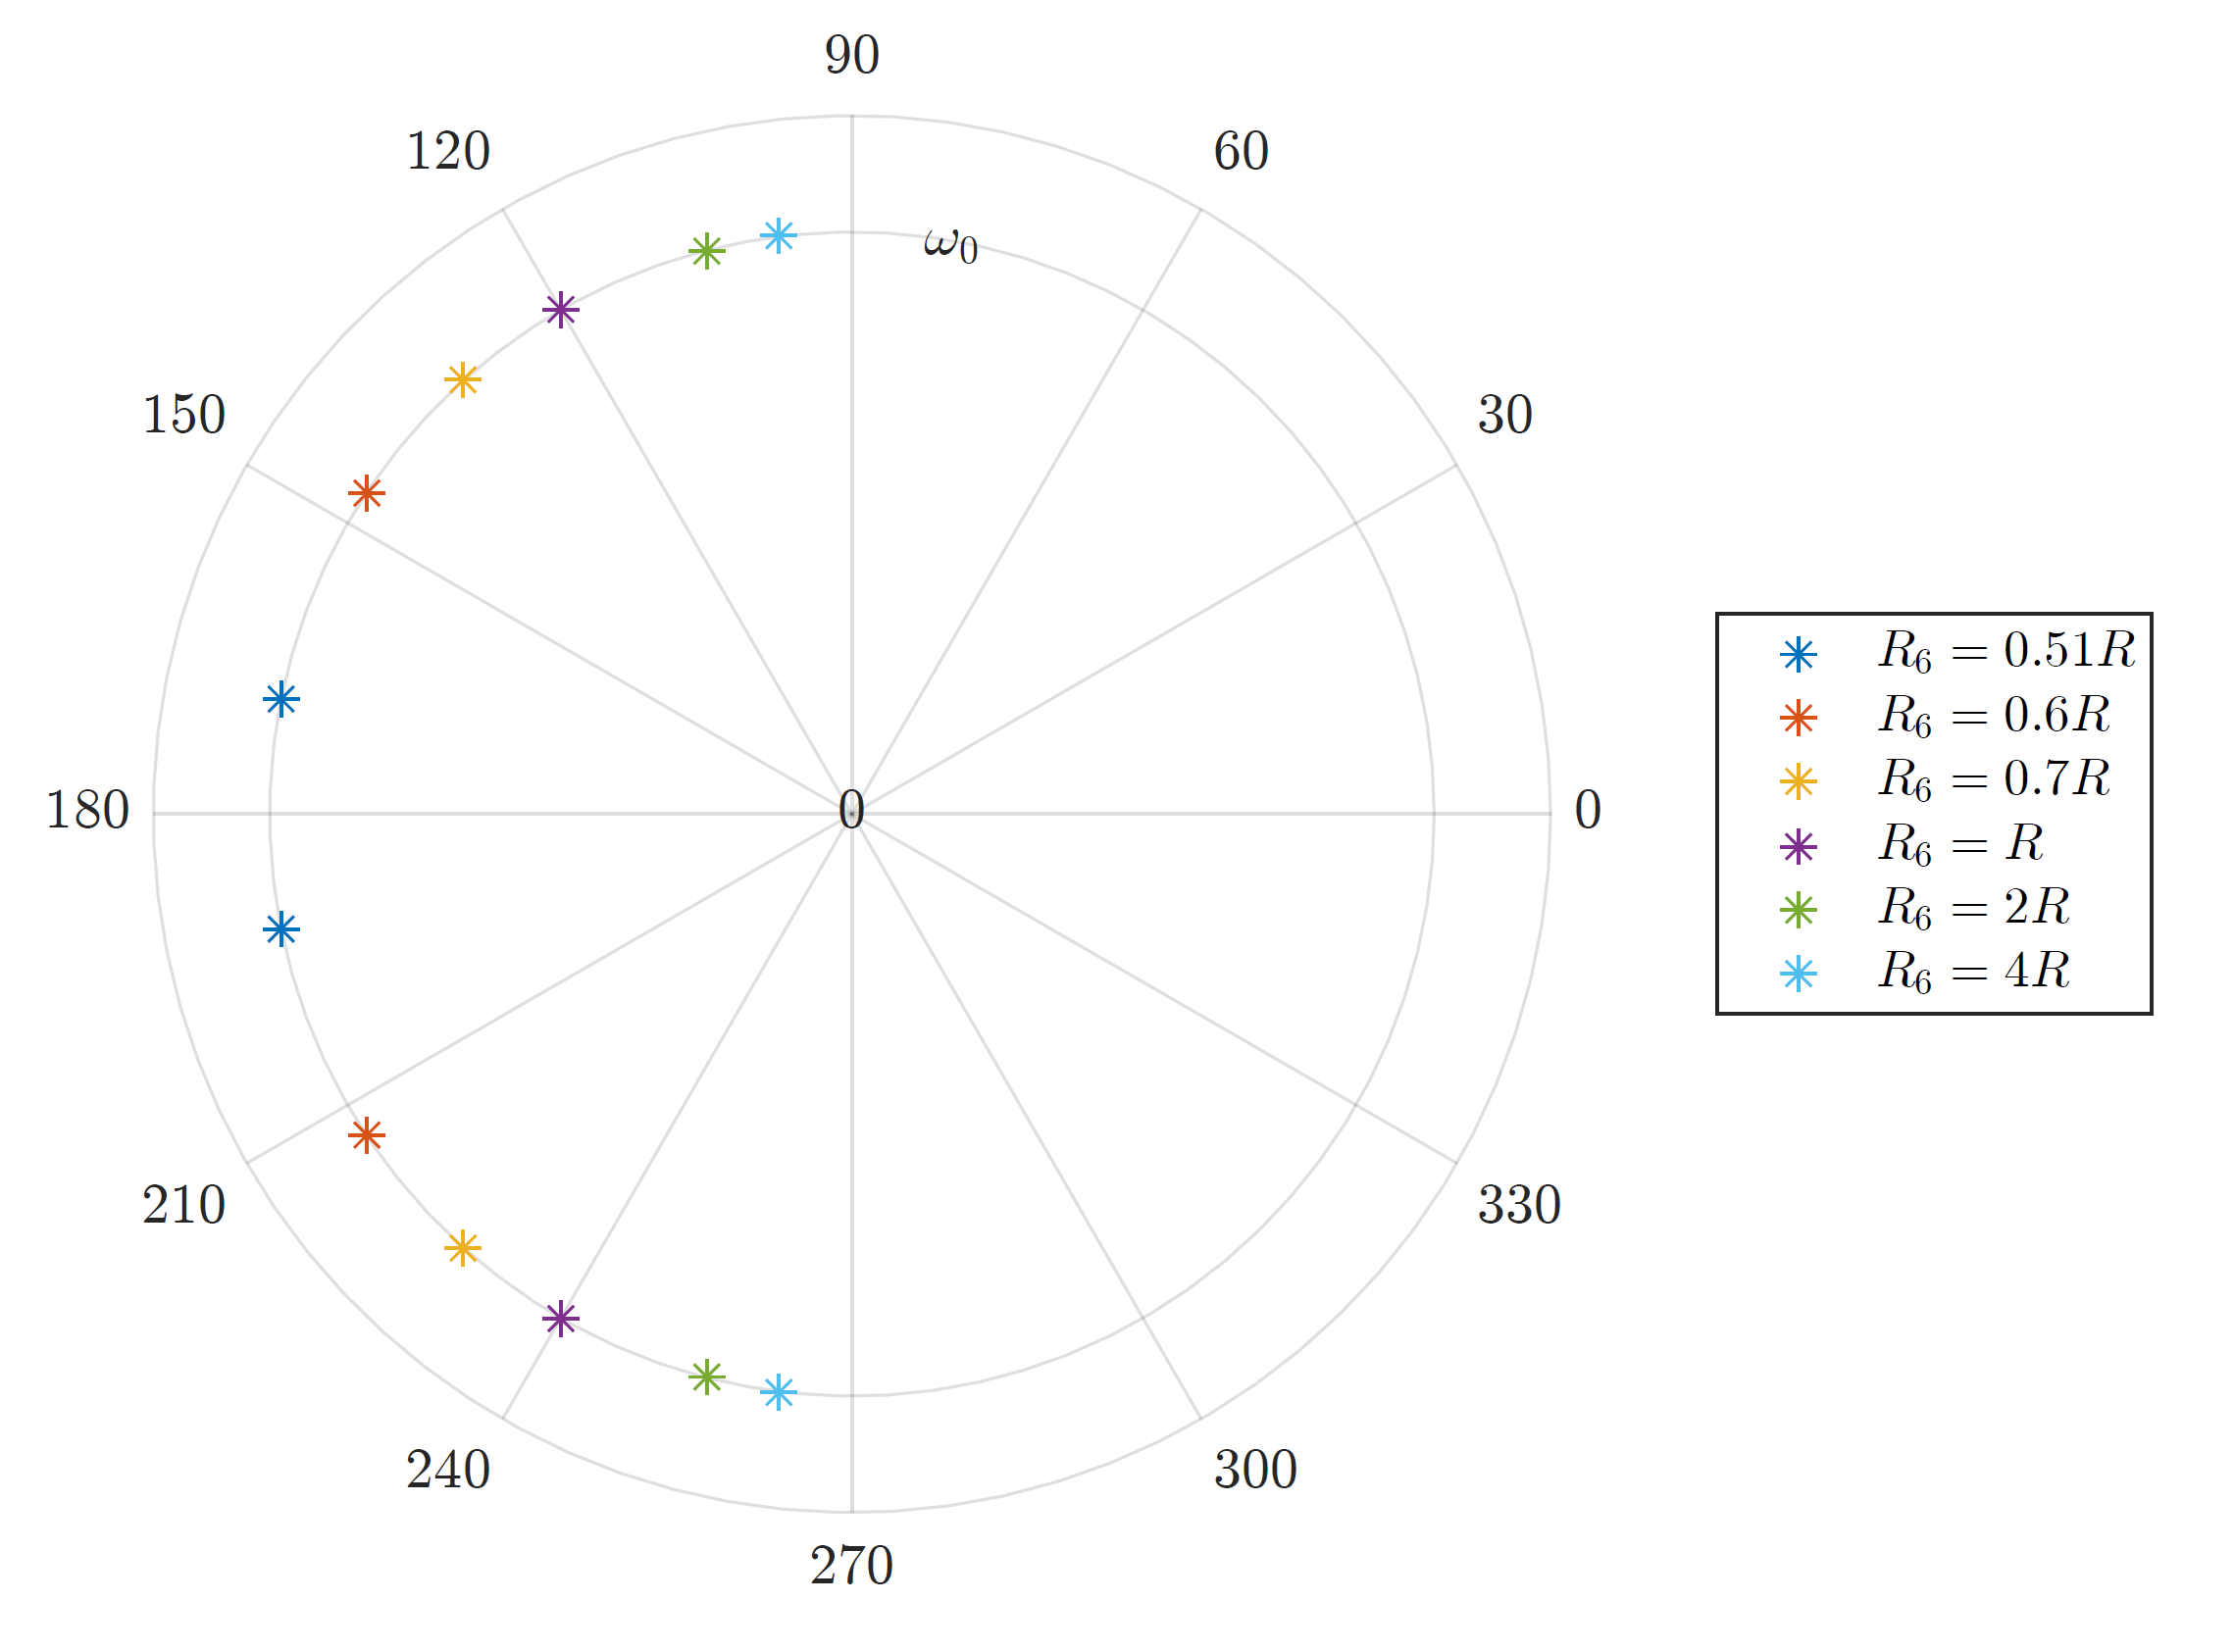
\includegraphics[scale=0.5]{../parte1/informe/resources/1_polos_complejos}
\caption{Distribución de polos. Polos complejos conjugados}
\label{1_polos_complejos}
\end{figure}

\begin{figure}[ht]
\centering
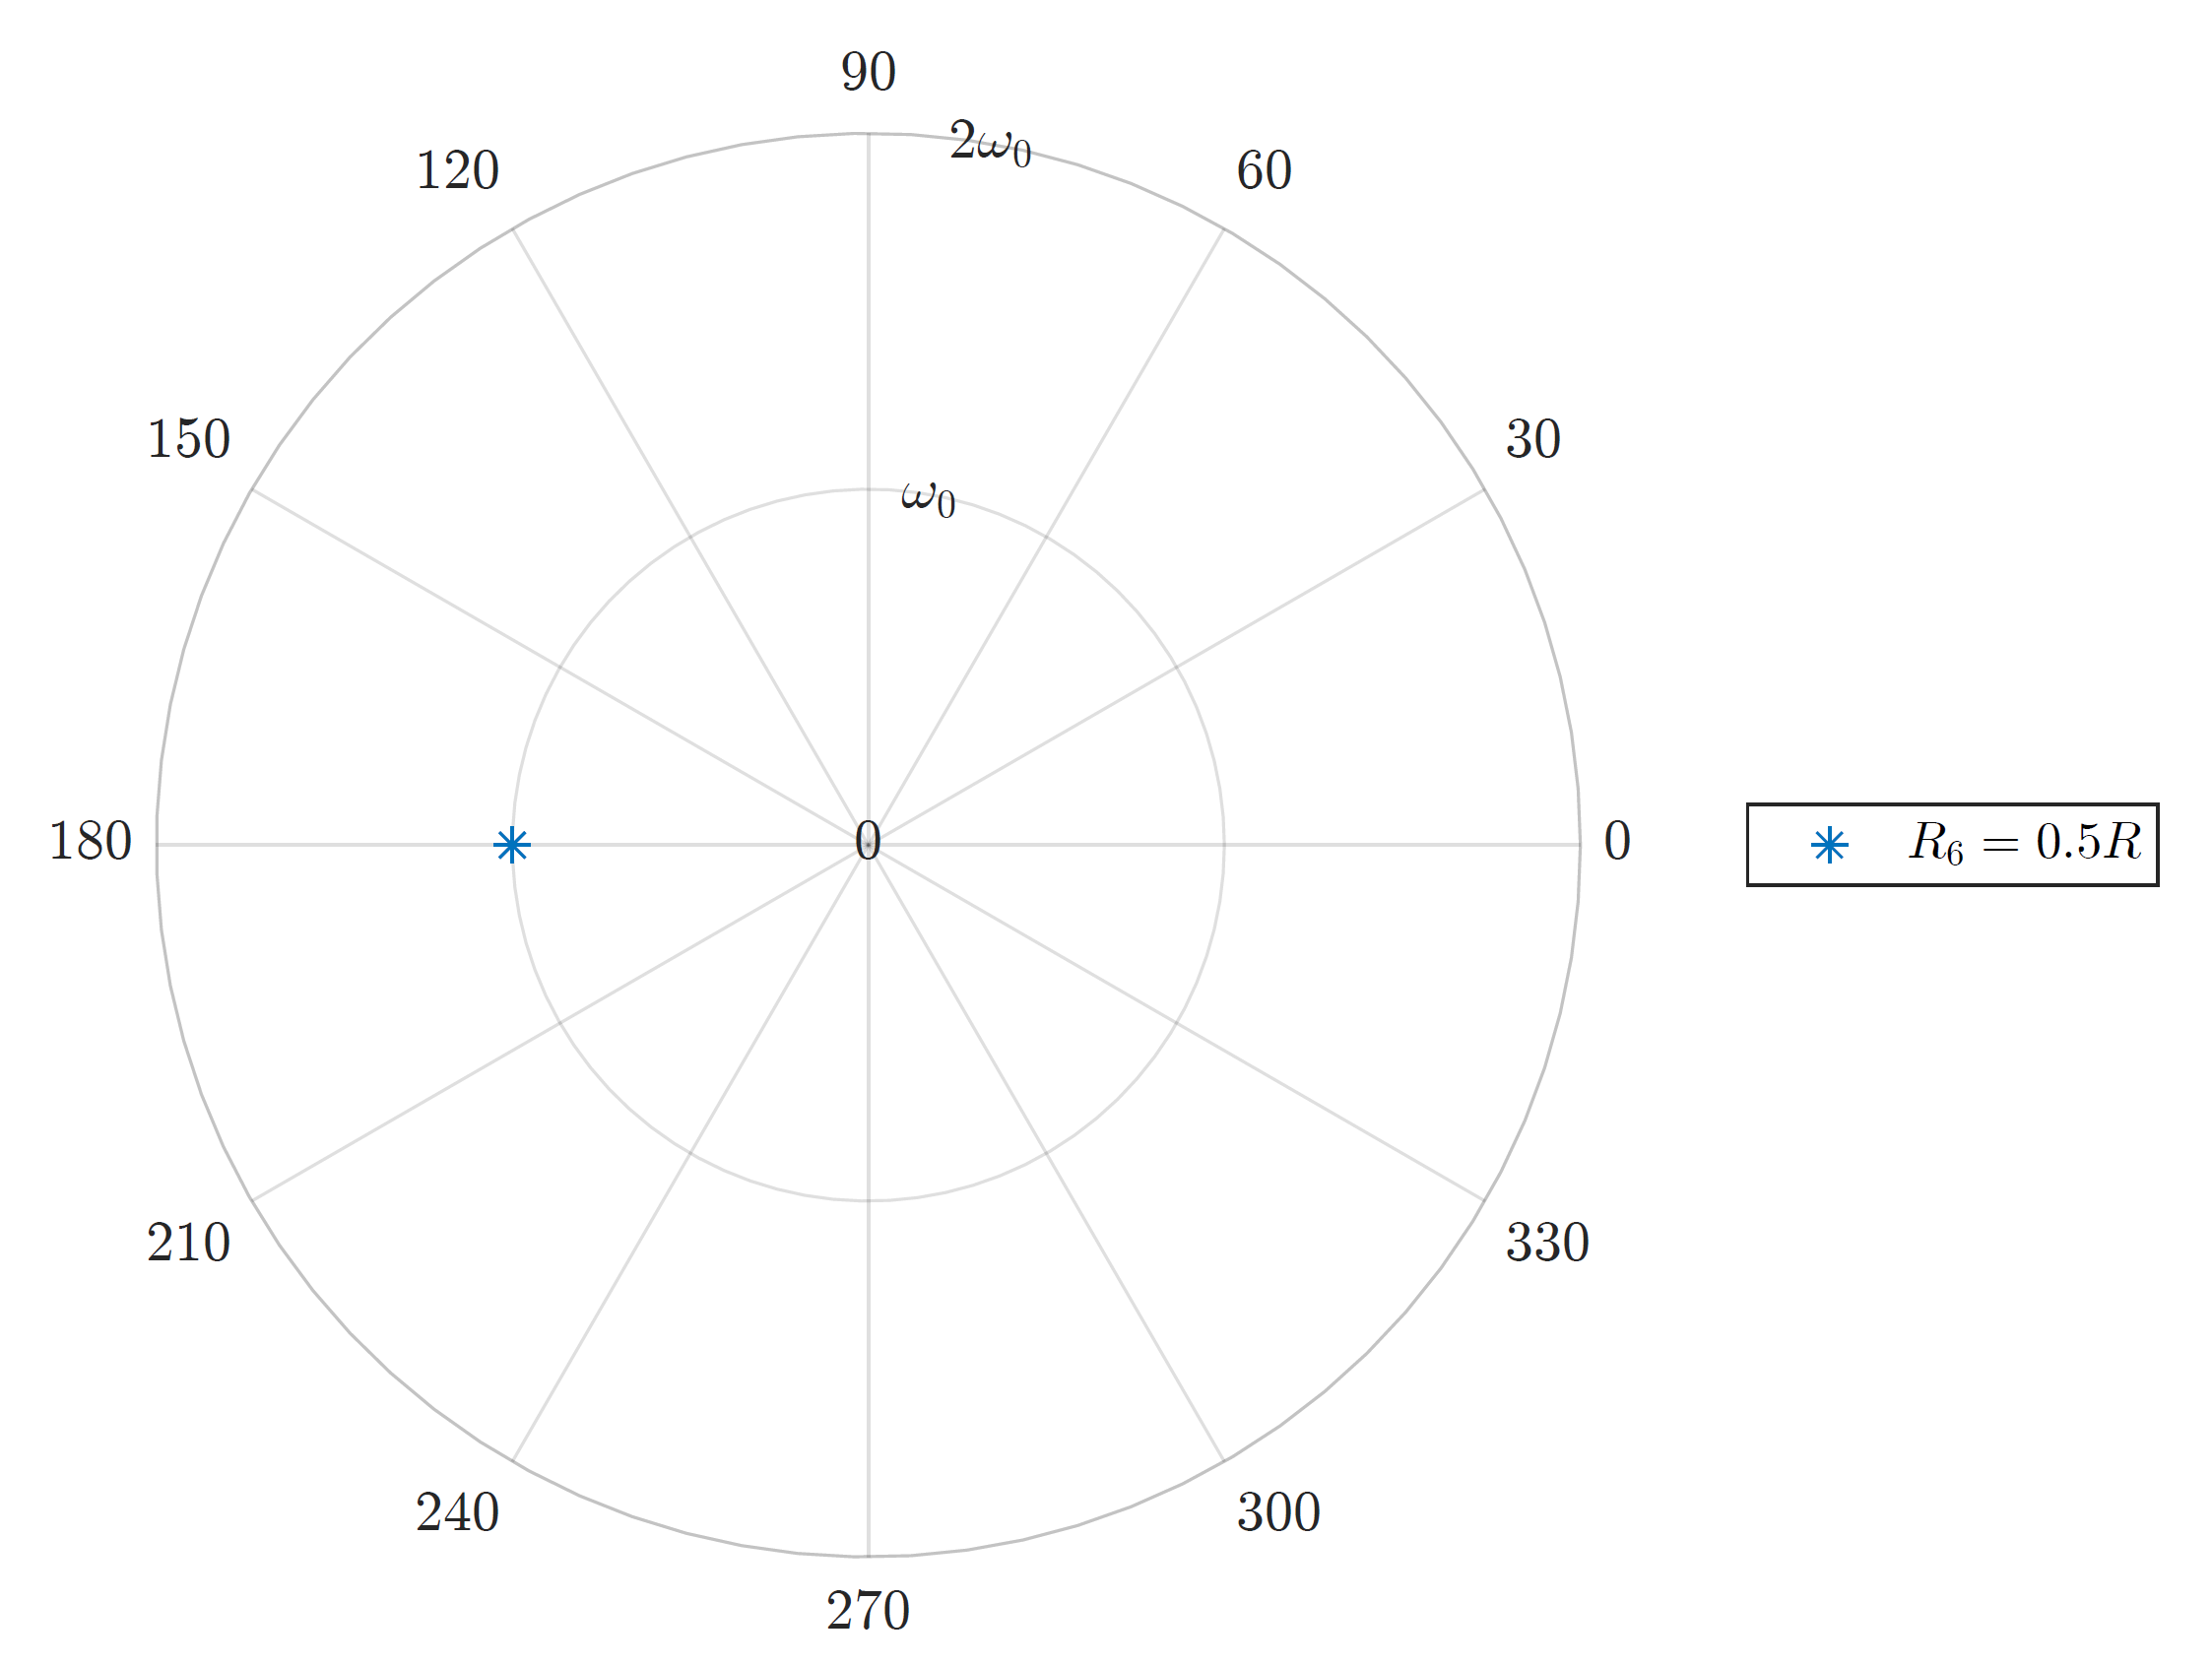
\includegraphics[scale=0.5]{../parte1/informe/resources/1_polo_doble}
\caption{Distribución de polos. Polo real doble}
\label{1_polo_doble}
\end{figure}

\subsubsection{Singularidades $R_6 \rightarrow \infty$, $R_6 \rightarrow 0$}
A partir de la Expresión \ref{exp_1_polos}, se tomó limite para los casos $R_6 \rightarrow \infty$, lo que implica $Q \rightarrow \inf$ y $R_6 \rightarrow 0$, que implica $Q \rightarrow 0$, por la relación $R_6 = QR$, dado que se asume $R$ un valor fijo finito. 

El caso singular $R_6 \rightarrow \infty$ genera una distribución de polos complejos conjugados ubicados sobre el eje imaginario y de magnitud $\omega_0$. $\$_{1,2} = \pm j\omega_0$. Esta tendencia puede observarse en la Figura \ref{1_polos_complejos}. 

Por otro lado, al $R_6$ aproximarse a 0, la distribución de polos de la transferencia esta caracterizada por un par de polos ubicados en la semirecta real negativa, de forma que tienden a alejarse a medida que $R_6$ se hace mas pequeño, la tendencia se manifiesta en la Figura \ref{1_polos_reales}.

\subsection{Análisis de sensibilidades}
Se realizó un análisis de sensibilidades para determinar la variación de los distintos parámetros relevantes del circuito respecto a variaciones en los distintos componentes. El estudio de sensibilidades del circuito permite seleccionar los componentes de forma tal que las variaciones de estos tengan la mínima repercusión posible sobre los parámetros del circuito. Se realizaron análisis de sensibilidades de la frecuencia central dle filtro($\omega_0$), el factor de calidad($Q$), y la transferencia en magnitud evaluada en la frecuencia central $\omega_0$($H(j\omega_0)$). Se define la sensibilidad de $y$ respecto de $x$ como $S_x^y$, y se calcula como

\[
S_x^y = \frac{\partial y}{\partial x} \frac{x}{y}
\]

\subsubsection{Sensibilidad de $\omega_0$}
La expresión de la frecuencia central $\omega_0$ en función de los componentes del circuito se determinó en la Sección \ref{section_transf_filtro}, y esta depende de los componentes $R_1$, $R_3$, $R_4$, $R_8$, $C_6$ y $C_2$. Aplicando el cálculo de la sensibilidad, se obtuvo:

\begin{subequations}
\begin{align*}
  S_{R_1}^{\omega_0} &= -1/2, &\text{Sensibilidad respecto de }R_1 \\
  S_{R_3}^{\omega_0} &= -1/2, &\text{Sensibilidad respecto de }R_3 \\
  S_{R_4}^{\omega_0} &= 1/2, &\text{Sensibilidad respecto de }R_4 \\
  S_{R_8}^{\omega_0} &= -1/2, &\text{Sensibilidad respecto de } R_8 \\
  S_{R_6}^{\omega_0} &= -1/2, &\text{Sensibilidad respecto de } R_6 \\
  S_{C_2}^{\omega_0} &= -1/2, &\text{Sensibilidad respecto de } C_2 \\
  S_{C_6}^{\omega_0} &= -1/2, &\text{Sensibilidad respecto de } C_6
\end{align*}
\end{subequations}

\subsubsection{Sensibilidad de $Q$}
En la Sección \ref{section_transf_filtro} se determinó la expresión del factor de calidad $Q$ del sistema,y a continuación se muestran los valores arrojados por el análisis de sensibilidades realizado sobre el mismo.

\begin{subequations}
\begin{align*}
  S_{R_1}^{Q} &= -1/2, &\text{Sensibilidad respecto de }R_1 \\
  S_{R_3}^{Q} &= -1/2, &\text{Sensibilidad respecto de }R_3 \\
  S_{R_4}^{Q} &= 1/2, &\text{Sensibilidad respecto de }R_4 \\
  S_{R_8}^{Q} &= -1/2, &\text{Sensibilidad respecto de } R_8 \\
  S_{R_6}^{Q} &= 1, &\text{Sensibilidad respecto de } R_6 \\
  S_{C_2}^{Q} &= 1/2, &\text{Sensibilidad respecto de } C_2 \\
  S_{C_6}^{Q} &= 1/2, &\text{Sensibilidad respecto de } C_6
\end{align*}
\end{subequations}

\subsubsection{Sensibilidad de $|H(j\omega_0)|$}
Al evaluar la Expresión \ref{1_transfer_completa} en $\$ = j\omega_0 = \sqrt{\frac{1}{L_{GIC}C_6}}$, se obtiene:

\[
|H(j\omega_0)| = \left(1 + \frac{R_4}{R_8}\right)
\]

Al calcular las sensibilidades respecto de $R_4$ y $R_8$, se obtuvo

\[
S_{R_4}^{|H(j\omega_0)|} = \left(1 + \frac{R_4}{R_8}\right)
\]
\[
S_{R_8}^{|H(j\omega_0)|} = -\left(1 + \frac{R_4}{R_8}\right)
\]

Al imponer $R_4 = R_8 = R$, se simplifica y se obtiene

\[
S_{R_4}^{|H(j\omega_0)|} = 2
\]
\[
S_{R_8}^{|H(j\omega_0)|} = -2
\]

\subsection{Selección de componentes}
A partir del análisis de sensibilidades realizado en le sección anterior, es posible establecer un criterio para la elección de componentes. Si se observan los valores obtenidos para las sensibilidades de $\omega_0$, se puede determinar que todos los componentes afectan al parámetro en cuestión practicamente en la misma proporción, por lo cual no es posible detectar un componente crítico a partir de estos resultados.

Al observar los resultados obtenidos para las sensibilidades del factor de calidad $Q$, se observa que variaciones en $R_6$ afectan en mayor proporción a $Q$ que variaciones en los restantes componentes. De esta forma, idealmente, se debería seleccionar un componente para $R_6$ con la menor desviación posible del valor teórico calculado para obtener los resultados deseados. Sin embargo, esta dinámica implicaría implementar las resistencias $R_1$, $R_3$, $R_4$ y $R_8$ mediante una combinación de resistores de valores comerciales,  lo cuál aumentaría las desviaciones que estas aportan. Es por esto que se decidió implementar la resistencia mas crítica(respecto al análisis de sensibilidades) mediante una combinación de resistores comerciales, y las resistencias que componen el GIC mediante un resistor comercial.

Se comienza por elegir un valor de $R$ que corresponda a un valor comercial re resitores de tolerancia de $5\%$, de forma que no requiera una combinación serie o paralelo implementarla. A partir del valor de $R$ establecido, se determina el valor de $R_6$. Luego, a partir del valor de la frecuencia central $\omega_0=13.000 rad/seg $ se determina el valor de $C$.

En los casos en que el valor calculado no coincide con un valor comericial para el componente en cuestión, de decidió utilizar como máximo 2 componentes combinados en serio o paralelo para lograr el valor mas próximo posible al calculado posible.
\smallskip

\begin{table}[h]
\centering
\begin{tabular}{|c|c|c|}
\hline 
Componente & Valor Calculado & Valor Utilizado \\ 
\hline 
$R_1$ & $3.3k\Omega$ & $3k\Omega$ \\ 
\hline 
$R_3$ & $3.3k\Omega$ & $3k\Omega$ \\
\hline 
$R_4$ & $3.3k\Omega$ & $3k\Omega$ \\ 
\hline 
$R_8$ & $3.3k\Omega$ & $3k\Omega$ \\ 
\hline 
$R_6$ & $13.2k\Omega$ & $13.2k\Omega$ \\
\hline 
$C_2$ & $23.31nF$ & $23.48nF$ \\
\hline 
$C_6$ & $23.31nF$ & $23.48nF$ \\
\hline 
\end{tabular} 
\caption{Valores de componentes calculados y utilizados}
\end{table}

Los valores de componentes seleccionados producen un filtro pasa banda con frecuencia central $\omega_0 = 12906 rad/seg$. Este valor representa un error porcentual del $7.24\%$ respecto de la frecuencia central buscada inicialmente.

\subsection{Distribución de las singularidades}
El análisis de sensibilidades determina que tanto varía el parámetro $Q$ respecto a variaciones en los distintos componentes del sistema. Como muestra la Expresión \ref{exp_1_polos} el tipo y la ubicación de los polos del sistema están ligados al valor de $Q$. De esta forma, conociendo la sensibilidad del parámetro en cuestión, y el valor de $Q$ y del componente que impone la mayor sensibilidad, se puede determinar los valores máximos y mínimos de $Q$, y así determinar la ubicación de los polos en los casos extremos de mayor desviación del valor central.

\[
Q_{max} = 4.4
\]

\[
Q_{min} = 3.6
\]

La Figura \ref{polos_sens_Q} muestra la distribución de las singularidades de la transferencia respecto a las variaciones que pueda sufrir el parámetro $Q$, considerando un valor de $R_6 = 13.2k\Omega$ y un valor de $Q_{central} = 4$.

\begin{figure}[H]
\centering
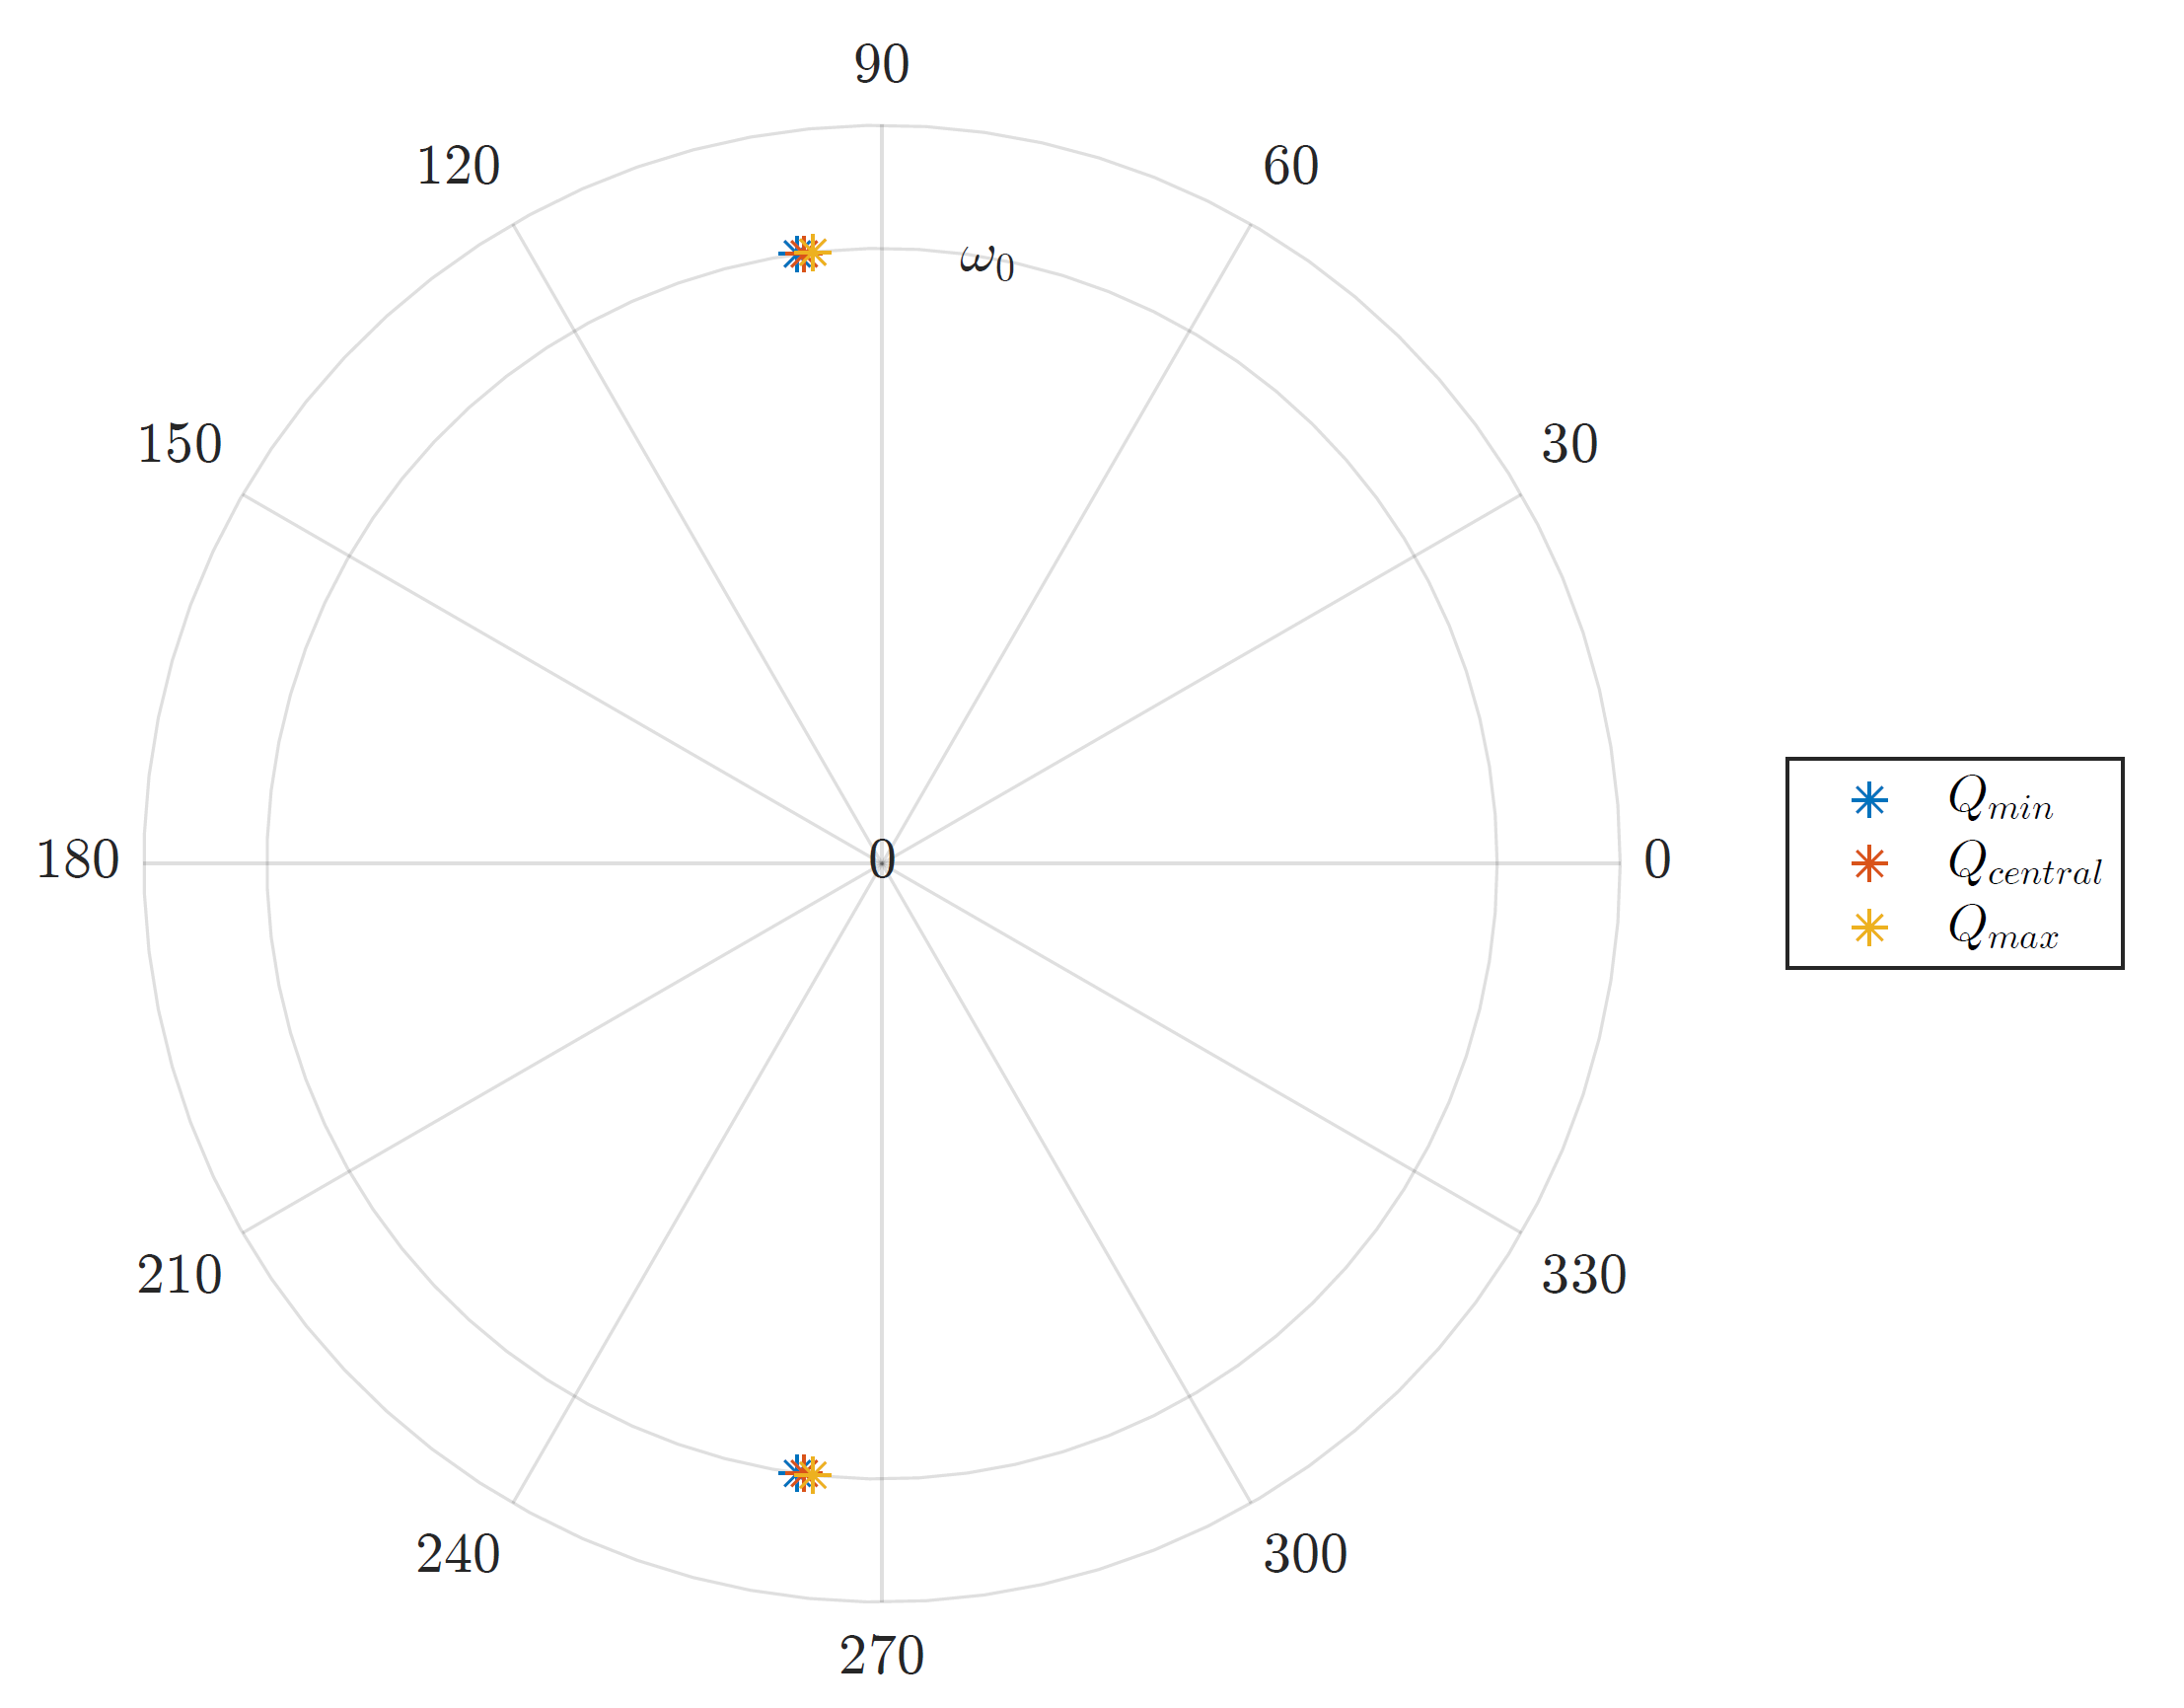
\includegraphics[scale=0.5]{../parte1/informe/resources/polos_sens_Q}
\caption{Dispersión de polos frente a variaciones de Q}
\label{polos_sens_Q}
\end{figure}

\subsection{Amplificadores operacionales compatibles}
El proceso de selección de amplificadores operacionales adecuados contempla determinar tres ítem a destacar:

\begin{enumerate}
\item Alta impedancia de entrada
\item Evitar Slew Rate
\item Evitar saturación
\end{enumerate}

Entre la amplia variedad de amplificadores operacionales disponibles en el mercado, se acotó el abanico de posibilidades a 3 integrados con características diferentes. Se realizó una preselección que incluyó los siguientes integrados: \emph{LM741}, \emph{TL082} y \emph{LM833}.

Para cada uno de los amplificadores operacionales se confeccionó un gráfico con las curvas de tensión de entrada máximo en función de la frecuencia debido a la tensión de saturación (tomando como tensión de alimentación $\pm 15V$ para los 3 integrados) y debido al slew rate. 

Las limitaciones que estos dos fenómenos pudieran imponer sobre el restante operacional que forma parte del GIC no fueron consideradas, ya que la salida de este tiene una transferencia dada por la Expresión \ref{1_transf_op2}. La transferencia en magnitud de este operacional se muestra en la Figura, y se puede observar que su ganancia máxima no supera los 0dB, por lo tanto el operacional que, a lo sumo, se verá limitado por los fenómenos mencionados, es aquel del cual se toma la salida del filtro.

\begin{equation}
\frac{v_{opamp2}}{v_{in}}(\$) = \frac{-\$}{R_6RC^2\$^3 + R_6C\$^2 + \frac{R_6}{R}\$}
\label{1_transf_op2} 
\end{equation}

\begin{figure}[H]
\centering
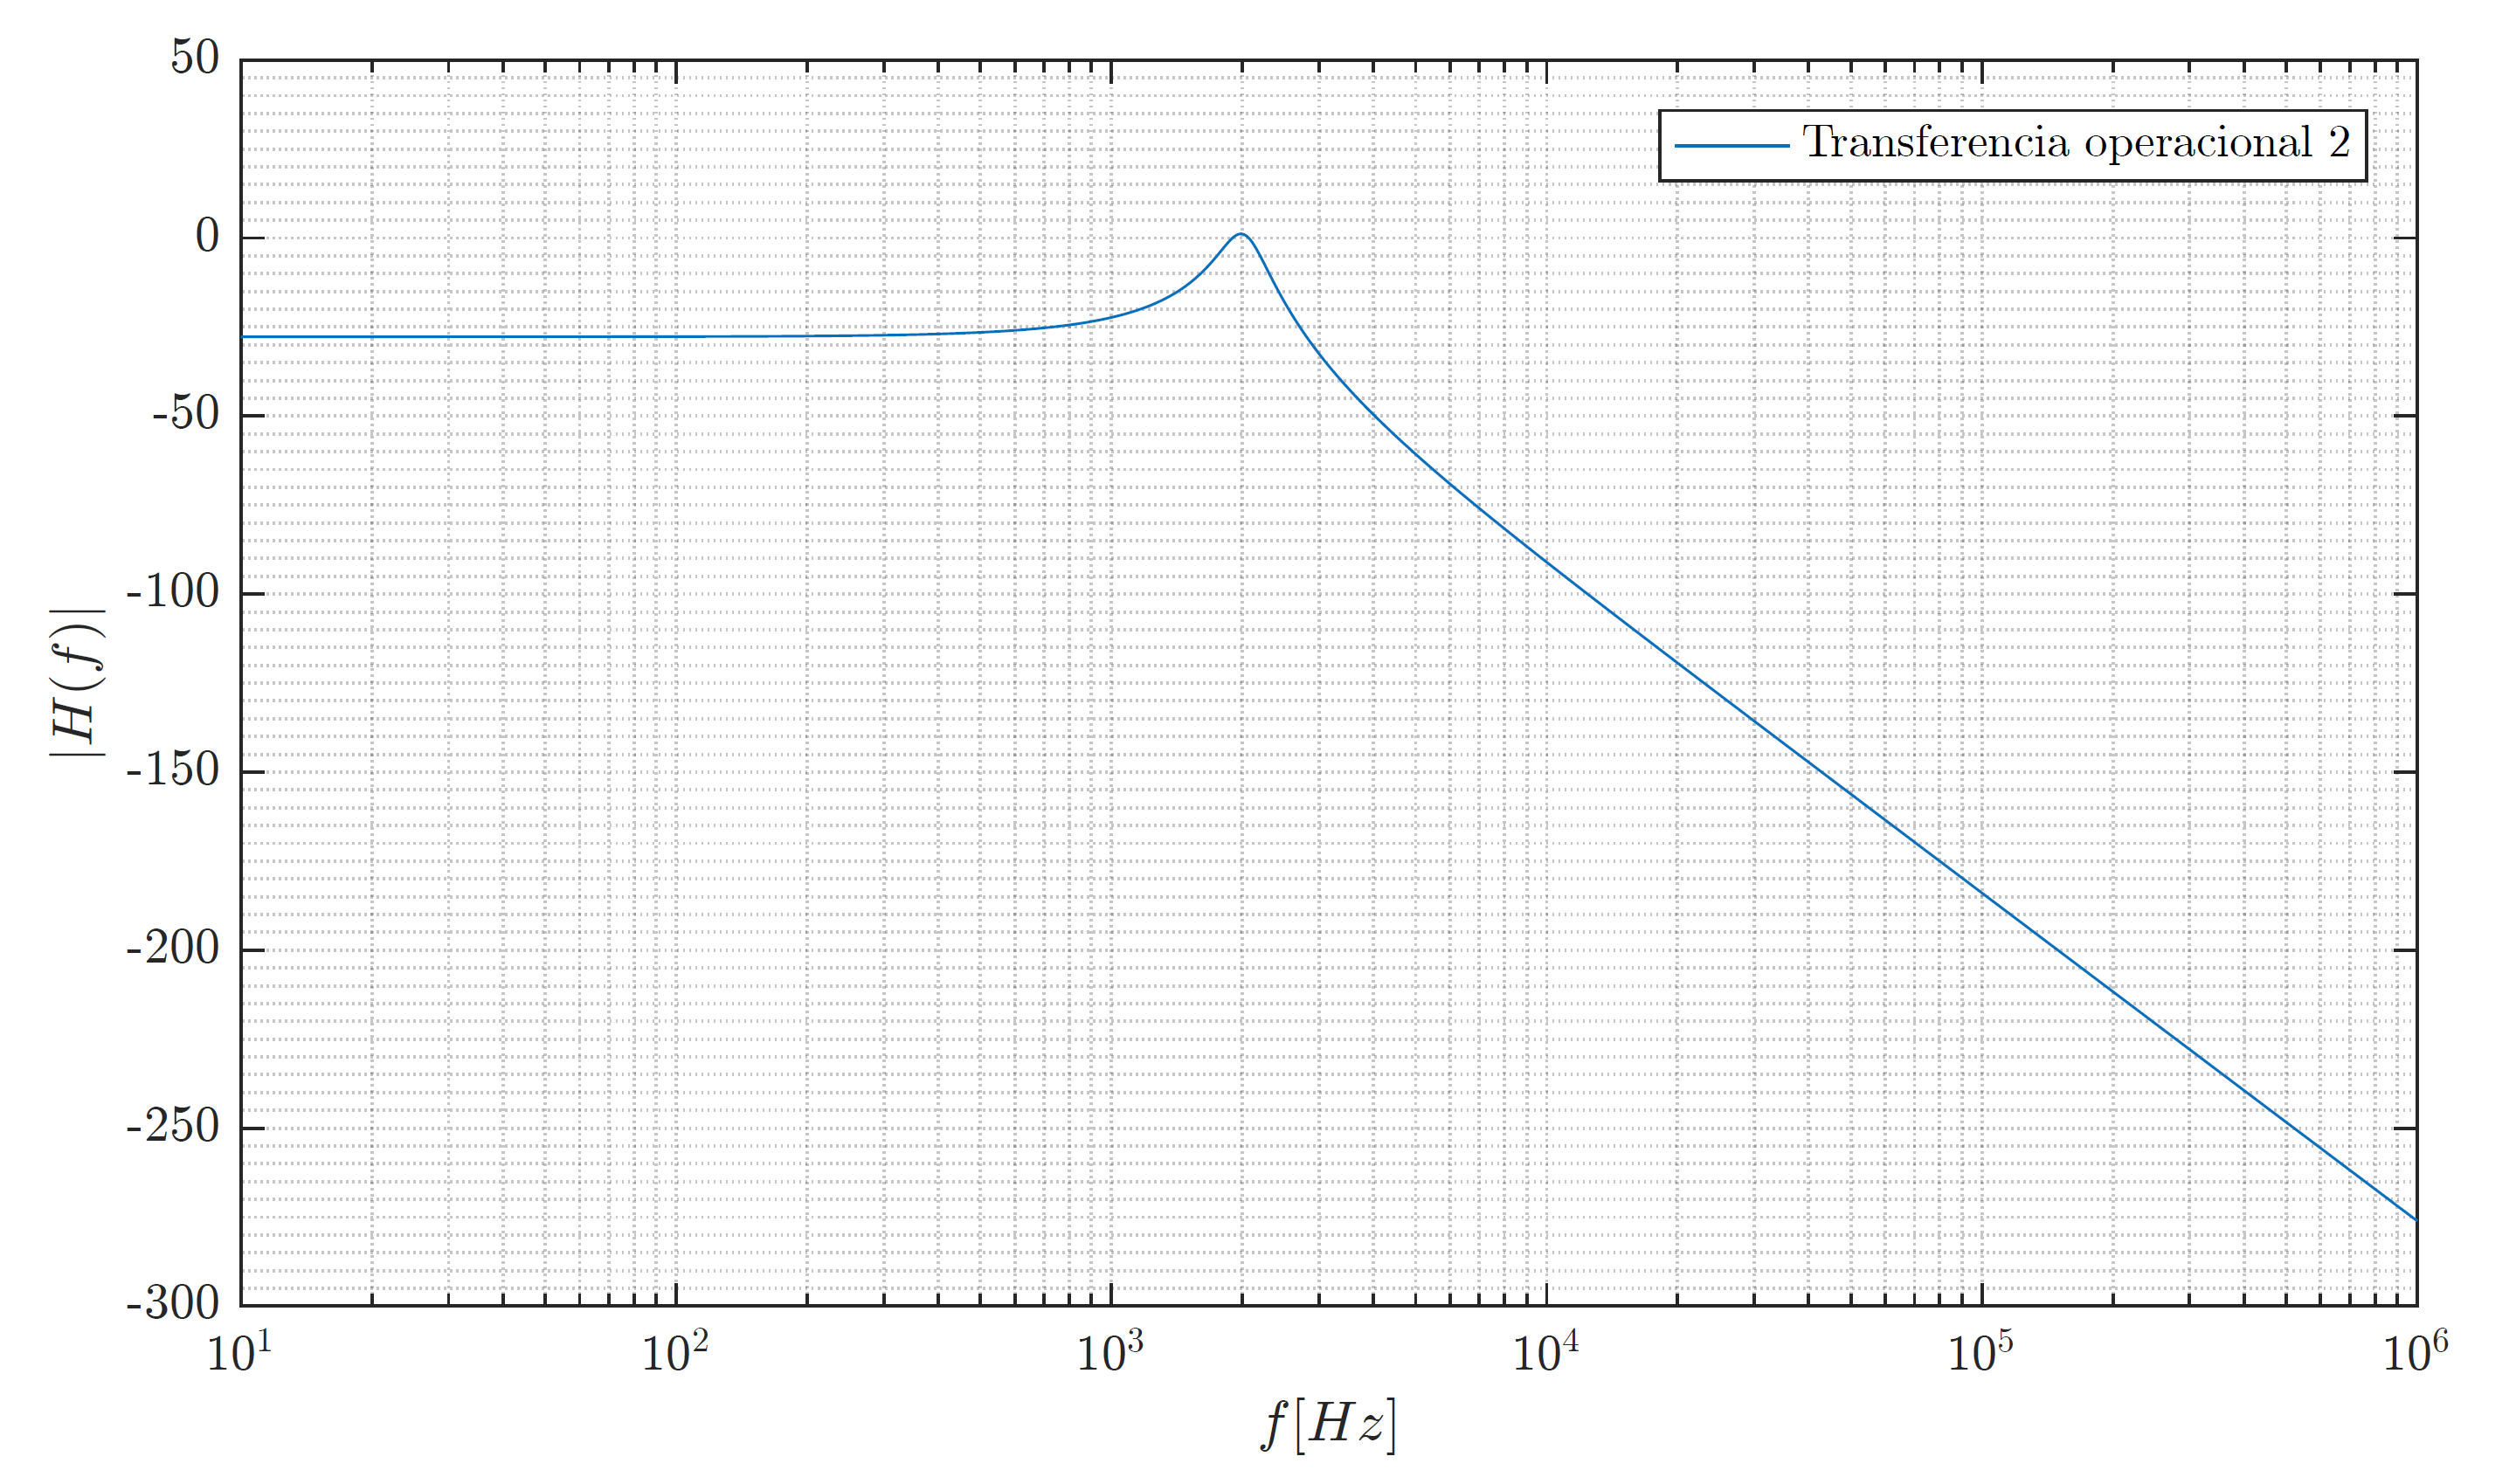
\includegraphics[scale=0.4]{../parte1/informe/resources/bode_segundo_opamp}
\label{1_bode_opamp2}
\caption{Transferencia en magnitud a la salida del segundo operacional del GIC}
\end{figure}

Las figuras muestran las curvas mencionadas para los operacionales TL082, LM833 y LM741 respectivamente.

\begin{figure}[H]
\centering
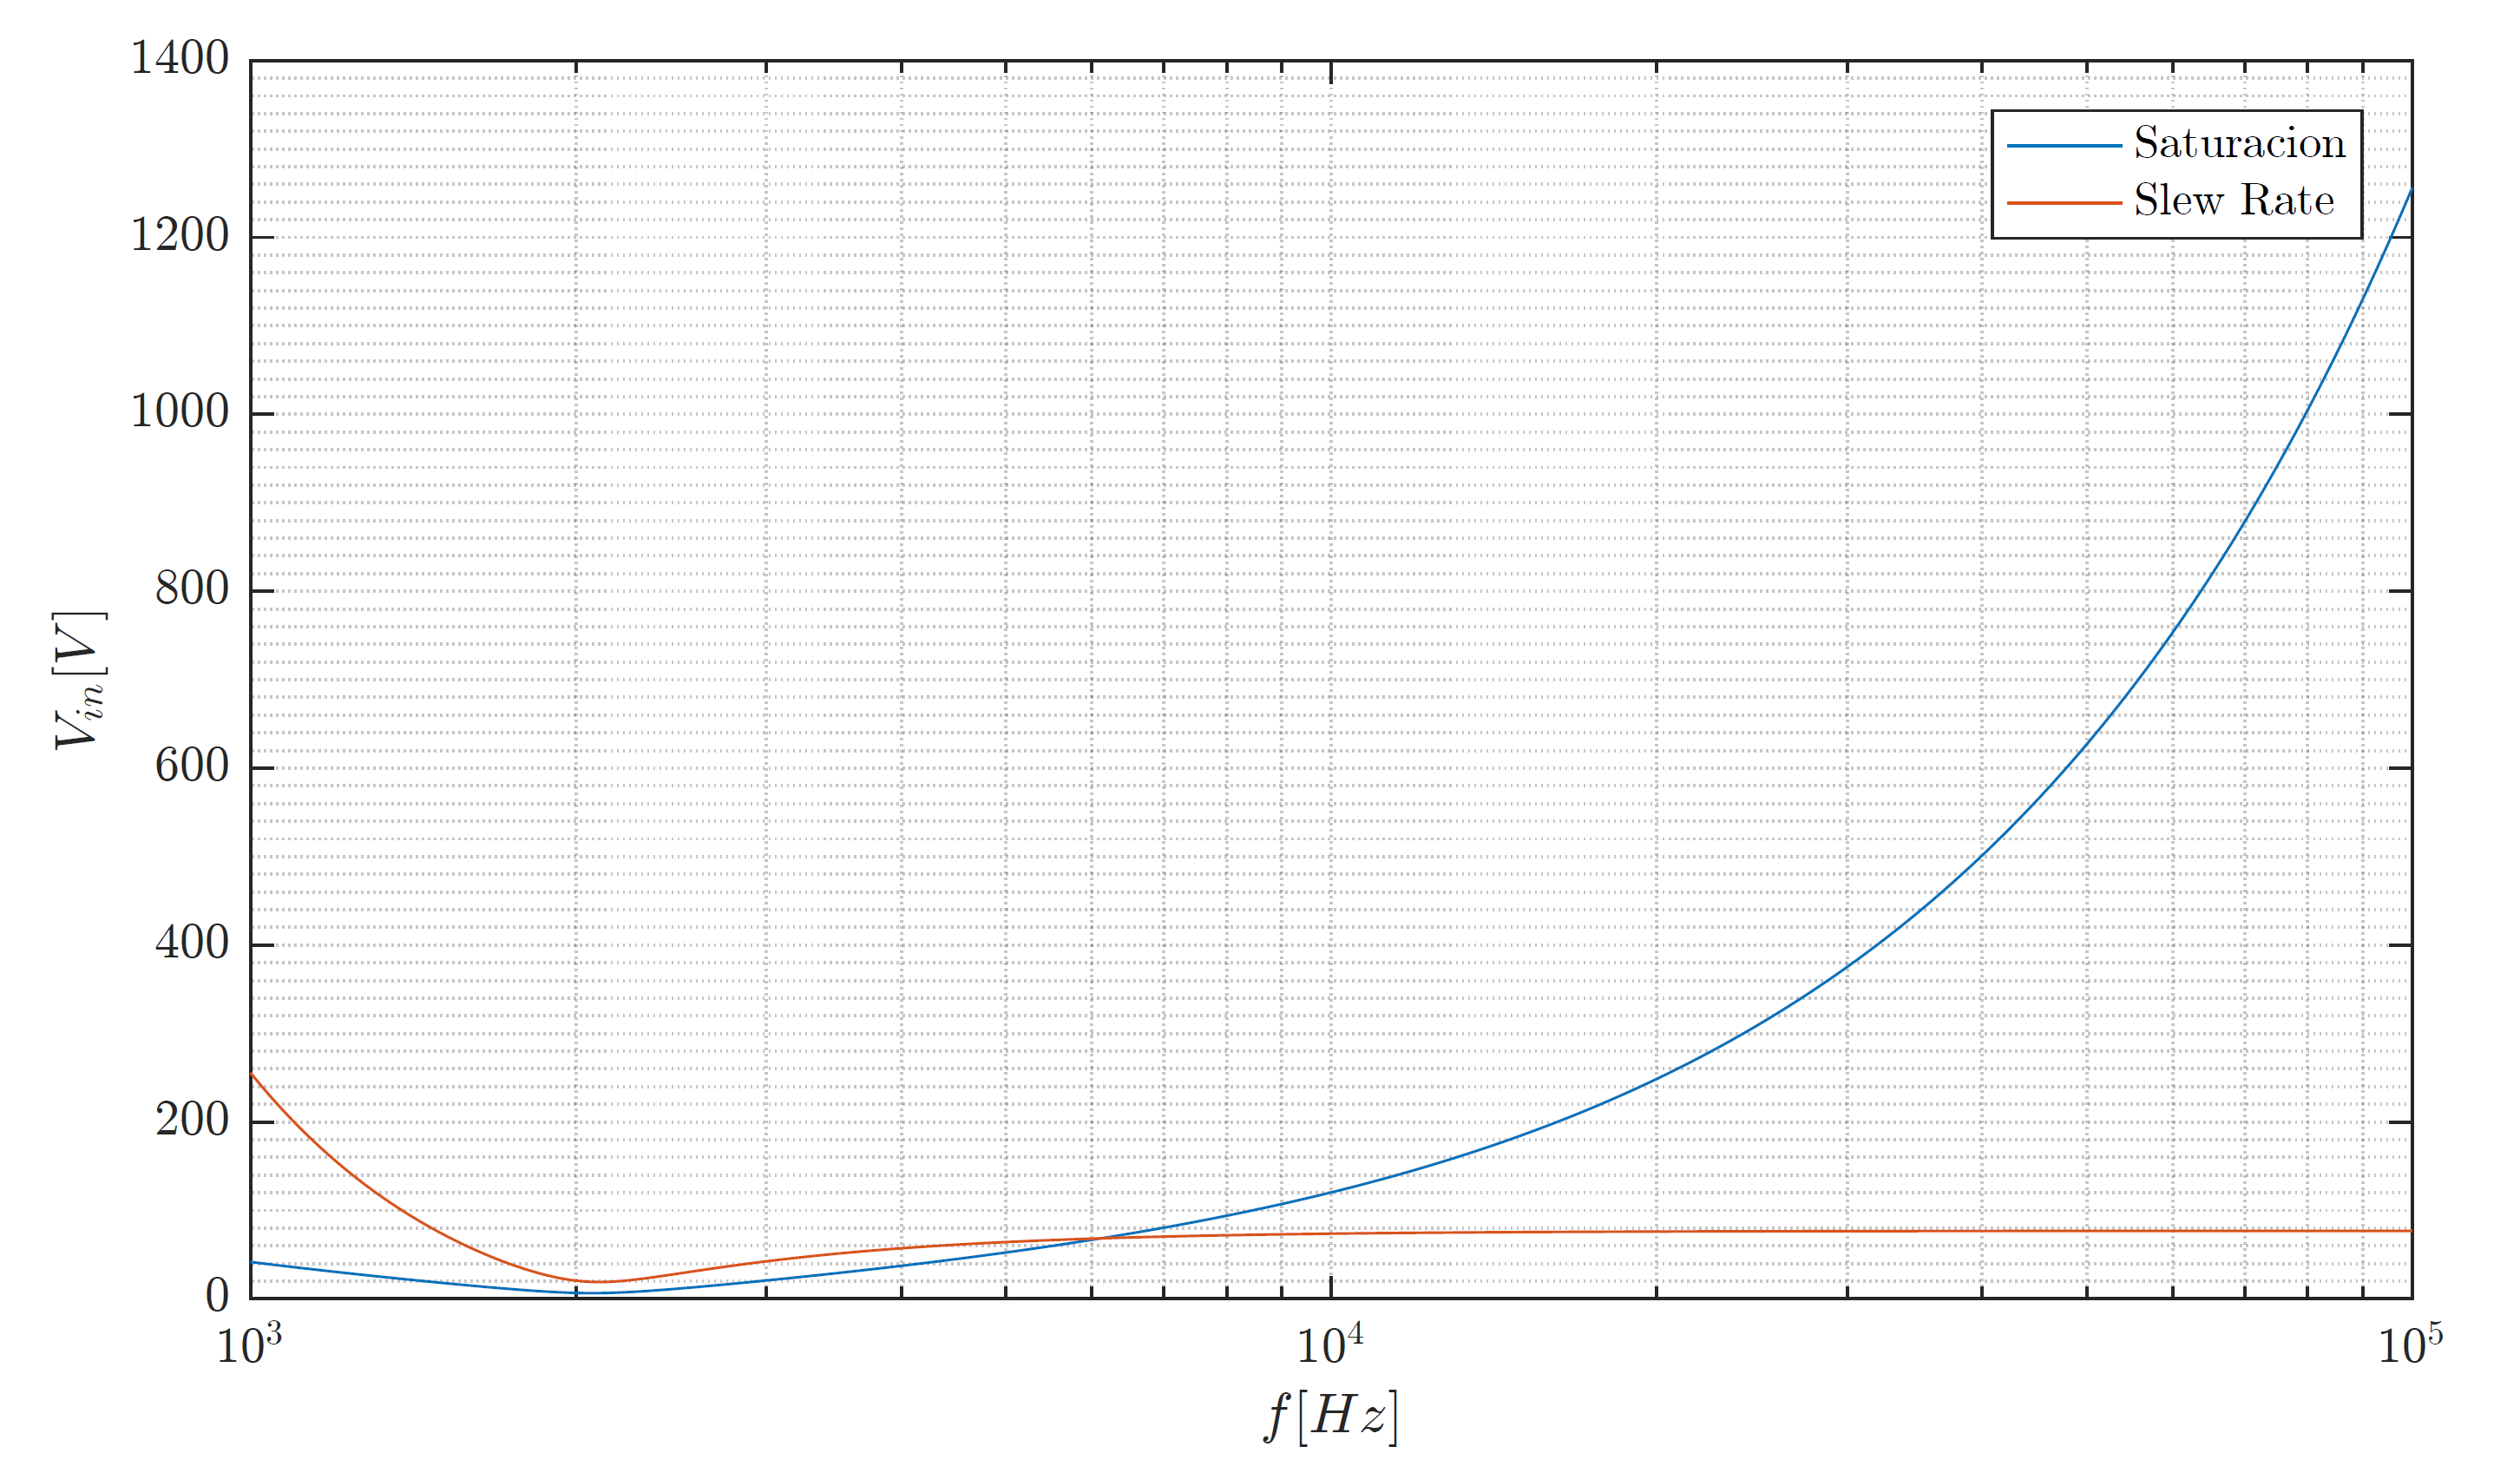
\includegraphics[scale=0.4]{../parte1/informe/resources/vin_max_LM741}
\label{1_vin_max_LM741}
\caption{Maxima tensión de entrada por saturación y slew rate para LM741}
\end{figure}

Se puede observar que en el caso del LM741, el slew rate impone un limite a la tensión de entrada inferior al limite por saturación del operacional en un rango de frecuencias en el cual, si bien la atenuación es muy grande, todavia se encuentra relativamente no tan alejado de la frecuencia central. Por este motivo se decidió descartar en primer lugar al operacional LM741.

\begin{figure}[H]
\centering
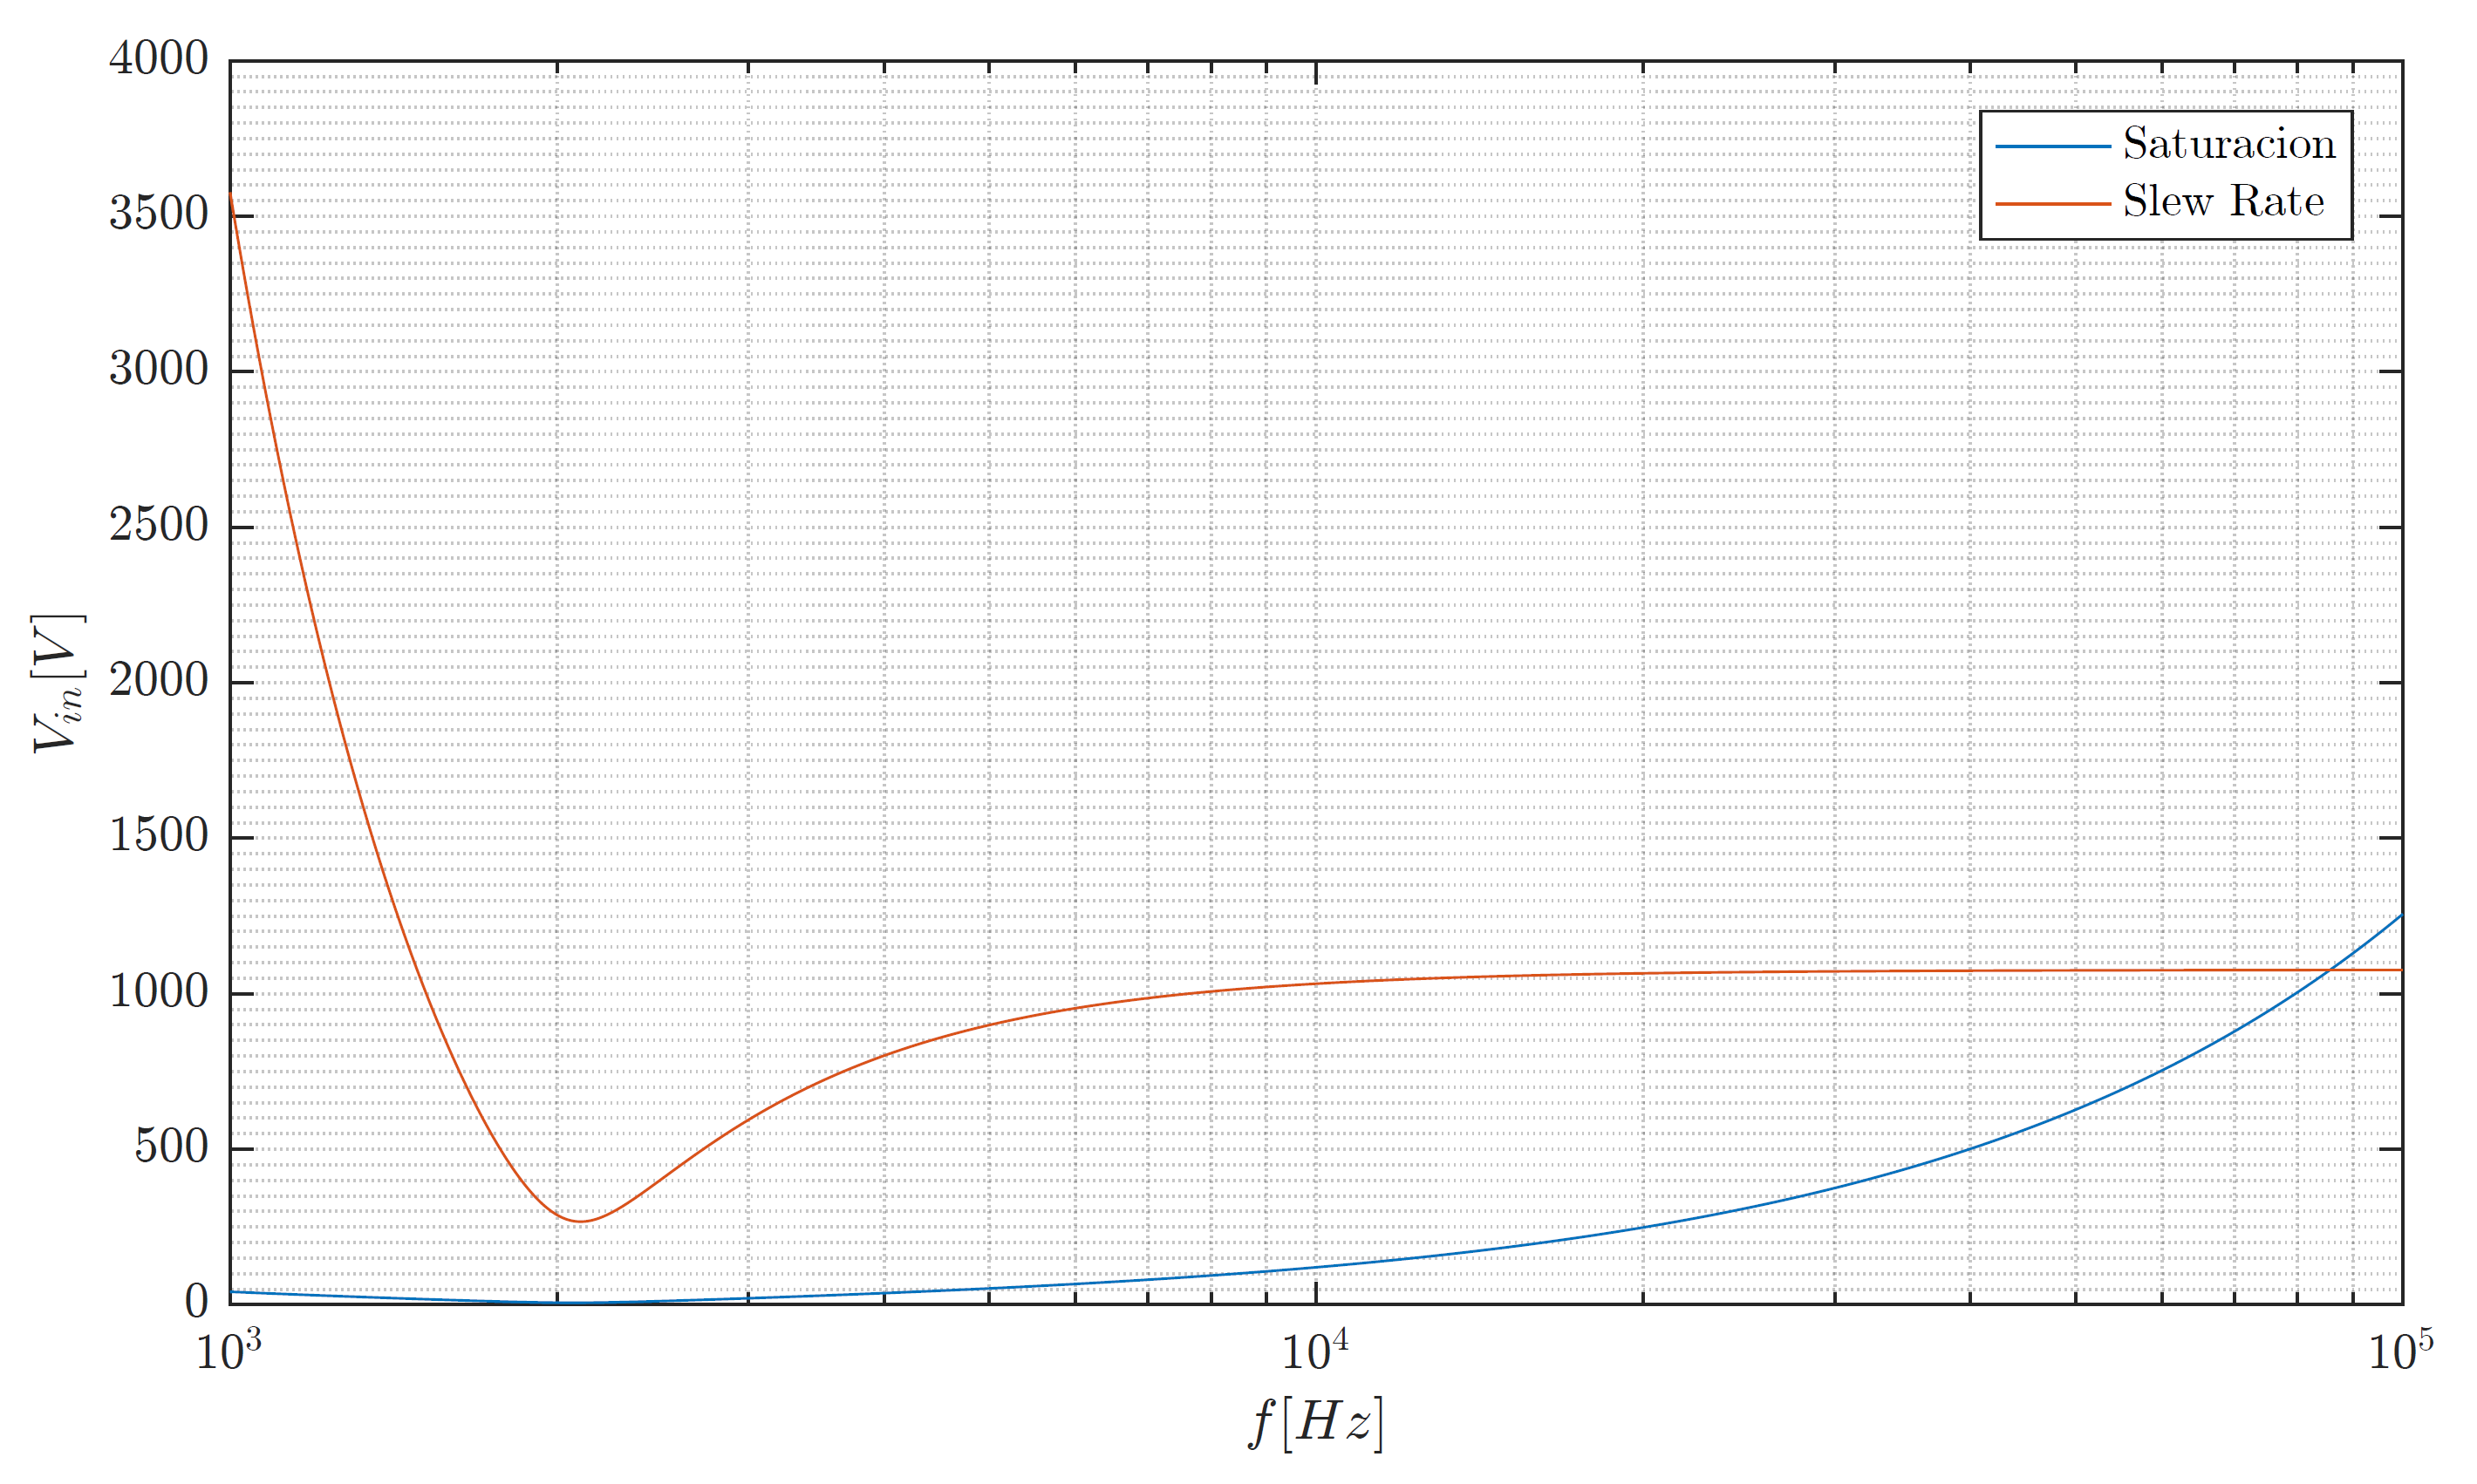
\includegraphics[scale=0.4]{../parte1/informe/resources/vin_max_LM833}
\label{1_vin_max_LM833}
\caption{Maxima tensión de entrada por saturación y slew rate para LM833}
\end{figure}

Respecto al operacional LM833, la distorsión por slew rate impone un limite para la tension de entrada inferior al limite por saturación recien en frecuencias próximas a los $100 kHz$. Si bien no se trata de una frecuencia excesivamente alta, el filtro atenúa aproximadamente unos $-85 dB$ o el equivalente de aproximadamente $6x10^-5$ veces, con lo cual, difícilmente se trate de una frecuencia dentro del rango de trabajo. Por este motivo es que se decidió no descartar el operacional Tl082.

\begin{figure}[H]
\centering
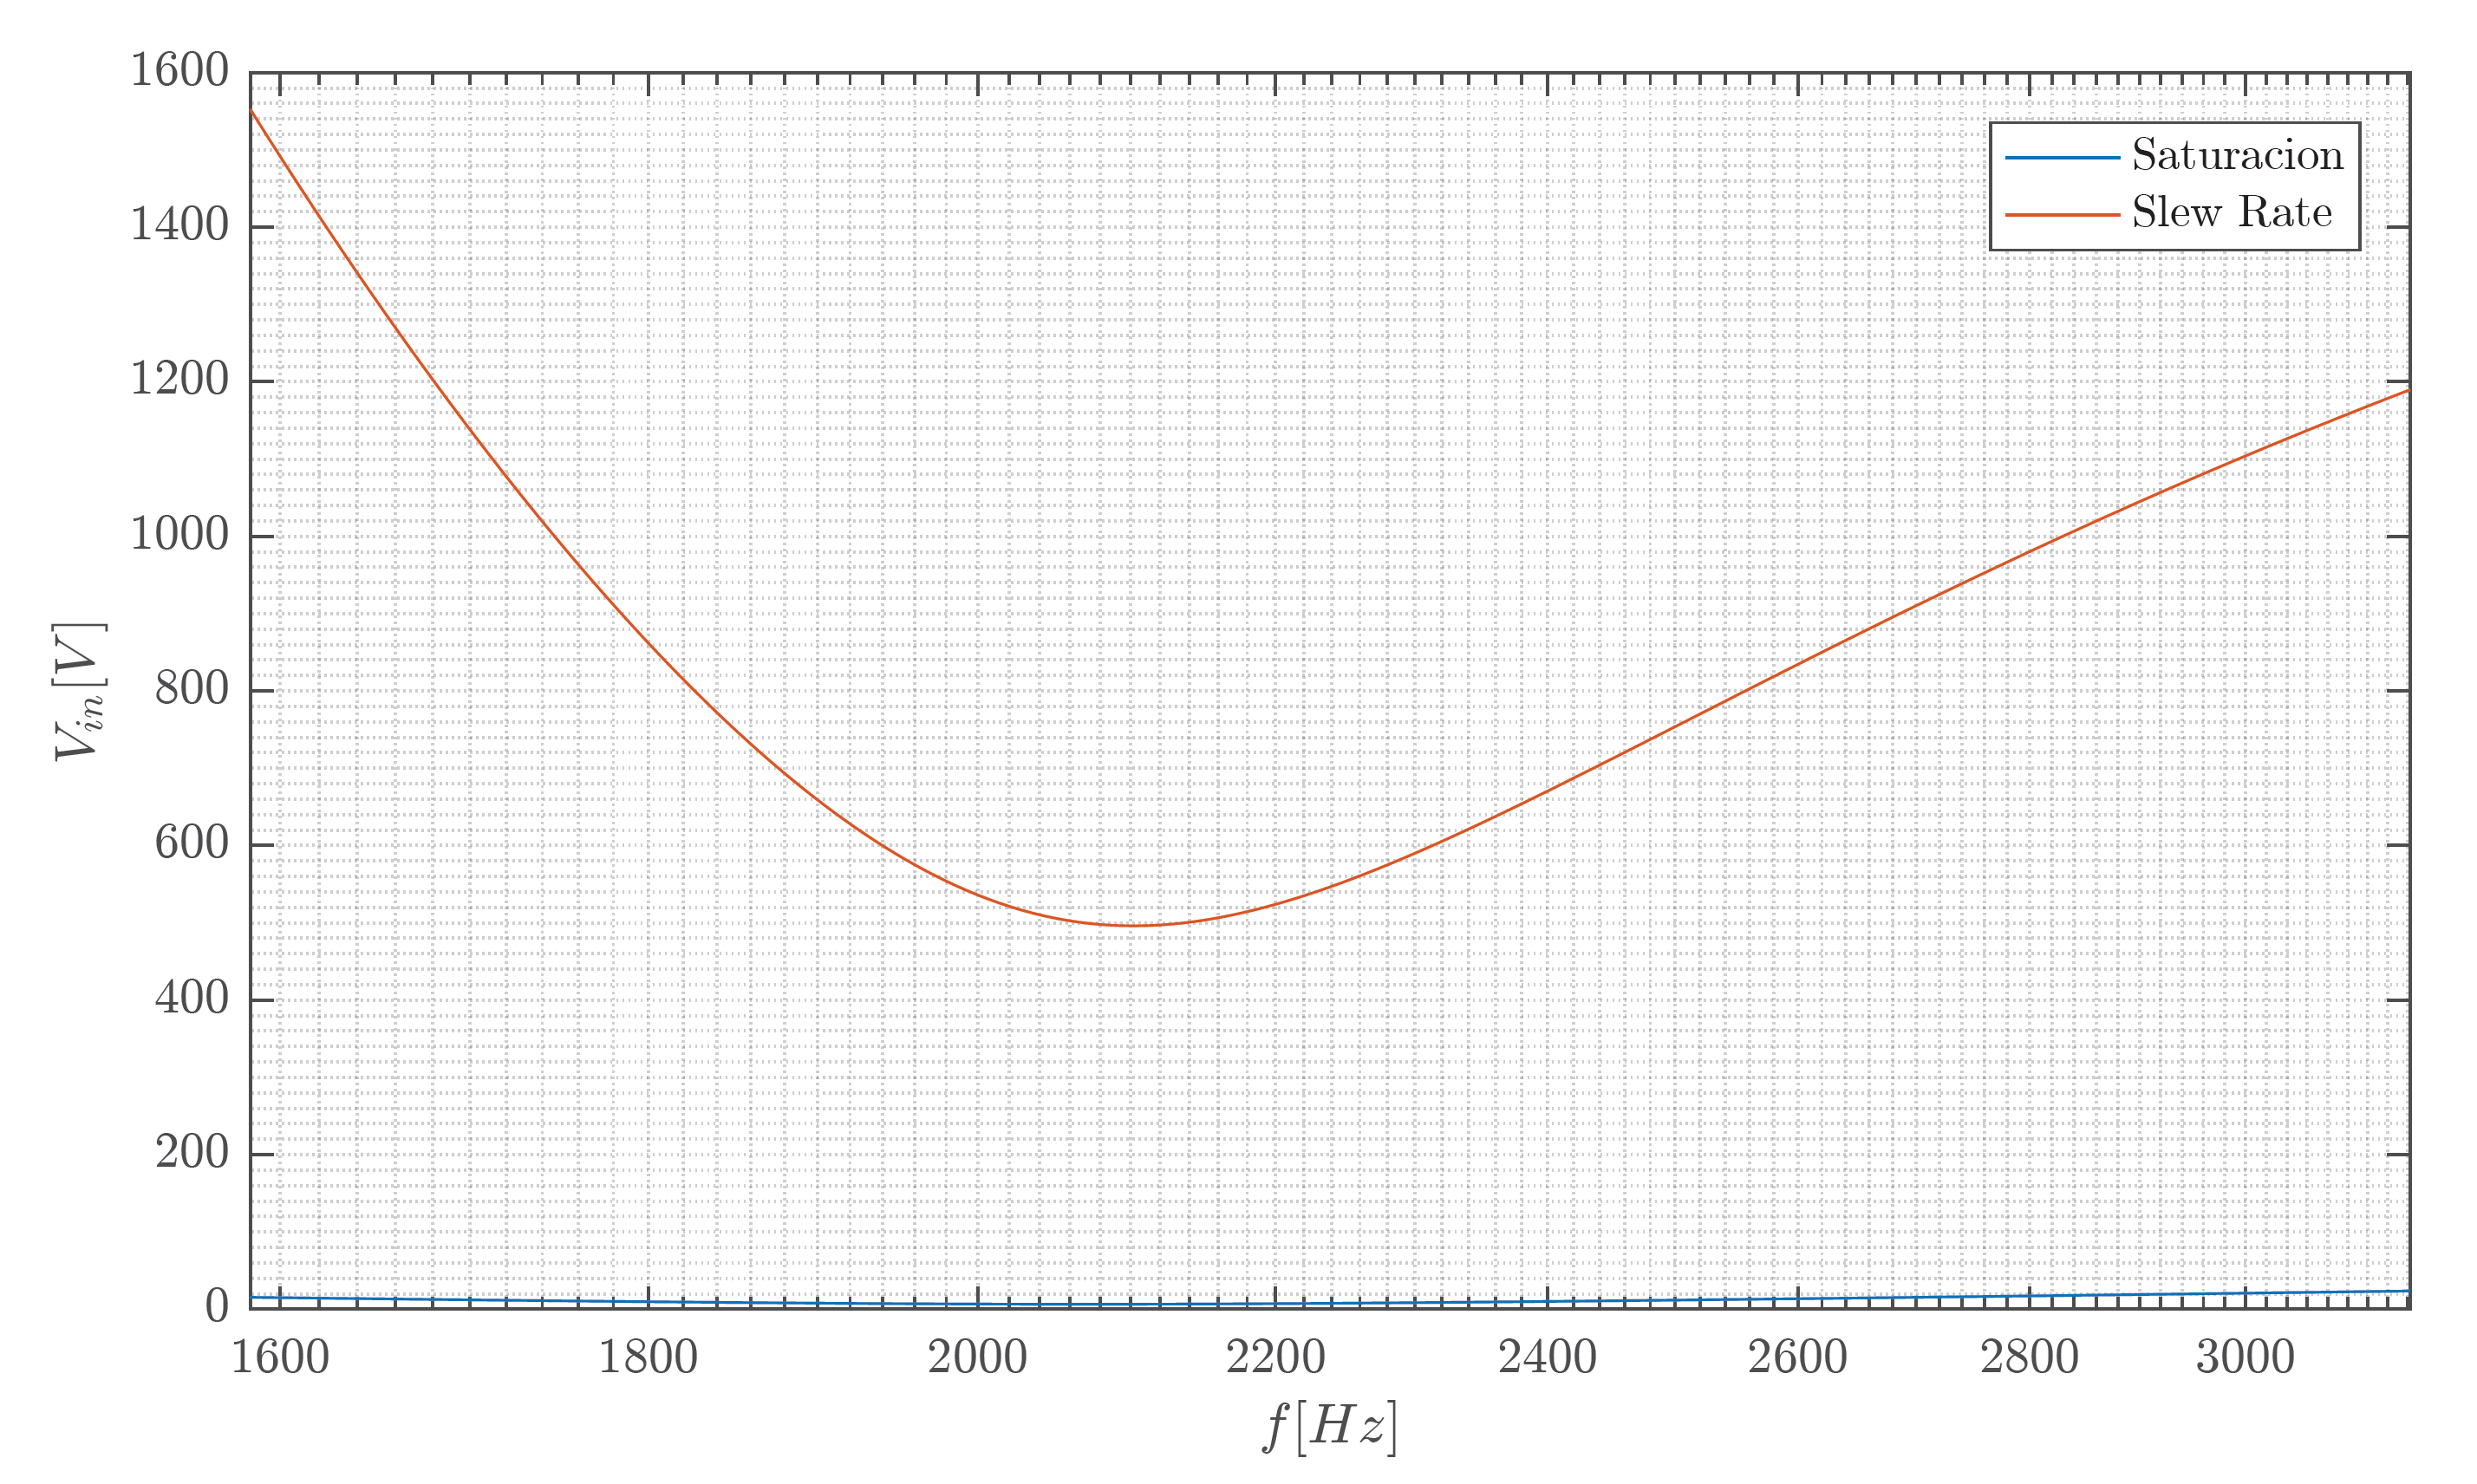
\includegraphics[scale=0.4]{../parte1/informe/resources/vin_max_TL082}
\label{1_vin_max_TL082}
\caption{Maxima tensión de entrada por saturación y slew rate para TL082}
\end{figure}

En el caso del TL082, se observa que la salida nunca podrá alcanzar un valor tal que su salida se vea distorsionada por slew rate sin antes verse afectada severamente por la saturación de alimentación. 

Si bien ambos operacionales, el LM833 y el TL082, son apropiados respecto a sus limitaciones por saturación y slew rate para implementar el filtro en cuestión, se decidió elegir el operacional LM833 debido a que este presenta una menor tensión de offset a la entrada y una menor distorsión armónica total (THD).

\section{Implementación}
\subsection{Circuito implementado}
\begin{figure}[ht]
\centering
\begin{circuitikz}[scale = 0.5, transform shape]

	\node [label=above:$v_{GIC}$](VGIC) at (0,0){};
	\node [below=4cm of VGIC](n1){};
	\node [below=1cm of n1](n2){};
	\node [below=1cm of n2](n3){};
	\node [below=1cm of n3](n3b){};
	\node [below=1cm of n3b](n4){};
	\node [below=1cm of n4](n5){};
	\node [below=1cm of n5](n6){};
	\node [below=1cm of n6](n7){};
	\node [below=1cm of n7](n8){};
	\node [below=1cm of n8](n9){};
	\node [below=1cm of n9](n10){};
	\node [below=1cm of n10](GND){};
	
	\node [left=2cm of VGIC](Vc){};
	\node [below=1.5cm of Vc] (Vc2){};
	\node [left=5cm of Vc, label=left:$v_{in}$](Vin){};
	
	\draw (Vin) to[R=$12k\Omega$,o-] ++(2.5,0) to[R=$1.2k\Omega$](Vc);
	\draw (Vc) to[C=$27nF$,*-] (Vc2);
	\draw (Vc2) to[C=$180nF$] ++(0,-1) node[ground]{};
	\draw (Vc) to[short, o-o] (VGIC);

	
	\node (Vp1) at ($(VGIC)!0.5!(n1)$){};
	\node (Vo2) at ($(n2)!0.5!(n3)$){};
	\node (Vn) 	at ($(n4)!0.5!(n5)$){};
	\node (Vo1) at ($(n6)!0.5!(n7)$){};
	\node (Vp2) at ($(n8)!0.5!(n9)$){};
	
	\node [right=1.5cm of Vp1](n11){};
	\node [right=1.5cm of Vn](n12){};
	\node [left=1cm of Vn](n13){};
	\node [left=1cm of Vp2](n14){};
		
	\node [right=3cm of Vo2](nop1){};
	\node [left=2.5cm of Vo1](nop2){};

	\draw (VGIC) to[short, o-] (n1);
	\draw (n1) to[R=$3.3k\Omega$,-] (n2);
	\draw (n2) to[short] (n3);
	\draw (n3) to[C=$27nF$,-] (n3b);
	\draw (n3b) to[C=$180nF$,-] (n4);
	\draw (n4) to[short] (n5);
	\draw (n5) to[R=$3.3k\Omega$,-] (n6);
	\draw (n6) to[short] (n7);
	\draw (n7) to[R=$3.3k\Omega$,-] (n8);
	\draw (n8) to[short] (n9);
	\draw (n9) to[R=$3.3k\Omega$,-] (n10);
	\draw (n10) to[short, -] (GND) node[ground]{};
	
	\draw (nop1) node[op amp,yscale=-1](amp1){};
	\draw (nop2) node[op amp,rotate=180,yscale=-1](amp2){};
	
	\draw (Vp1) to[short,*-] (n11);
	\draw (n11) to[short,-] (n11 |- amp1.+) to[short,-] (amp1.+);
	
	\draw (Vn) to[short,*-] (n12);
	\draw (n12) to[short,-] (n12 |- amp1.-) to [short,-] (amp1.-);	
	
	\draw (amp1.out) to[short,-] ++(1,0) coordinate (right_amp1);
	\draw (right_amp1) to[short] (right_amp1 |- Vo1) to[short,-*] (Vo1);
	\draw (right_amp1) to[short, -o] ++(1,0) node[label=right:$V_{out}$](){};
	
	\draw (Vn) to[short,*-] (n13);
	\draw (n13) to[short,-] (n13 |- amp2.-) to [short,-] (amp2.-);	
	
	\draw (Vp2) to[short,*-] (n14);
	\draw (n14) to[short,-] (n14 |- amp2.+) to[short,-] (amp2.+);
	
	\draw (amp2.out) to[short,-] ++(-1,0) coordinate (right_amp2);
	\draw (right_amp2) to[short] (right_amp2 |- Vo2) to[short,-*] (Vo2);

\end{circuitikz}
\caption{Circuito implementado}
\label{1_circuito_implementado}
\end{figure}

Se implementó el circuito de la Figura \ref{1_circuito_implementado} en PCB, para medir sus parámetros característicos y ser contrastados con aquellos calculados. La Figura \ref{1_pcb} muestra el diseño final de la implementación. 

\begin{figure}[ht]
\centering
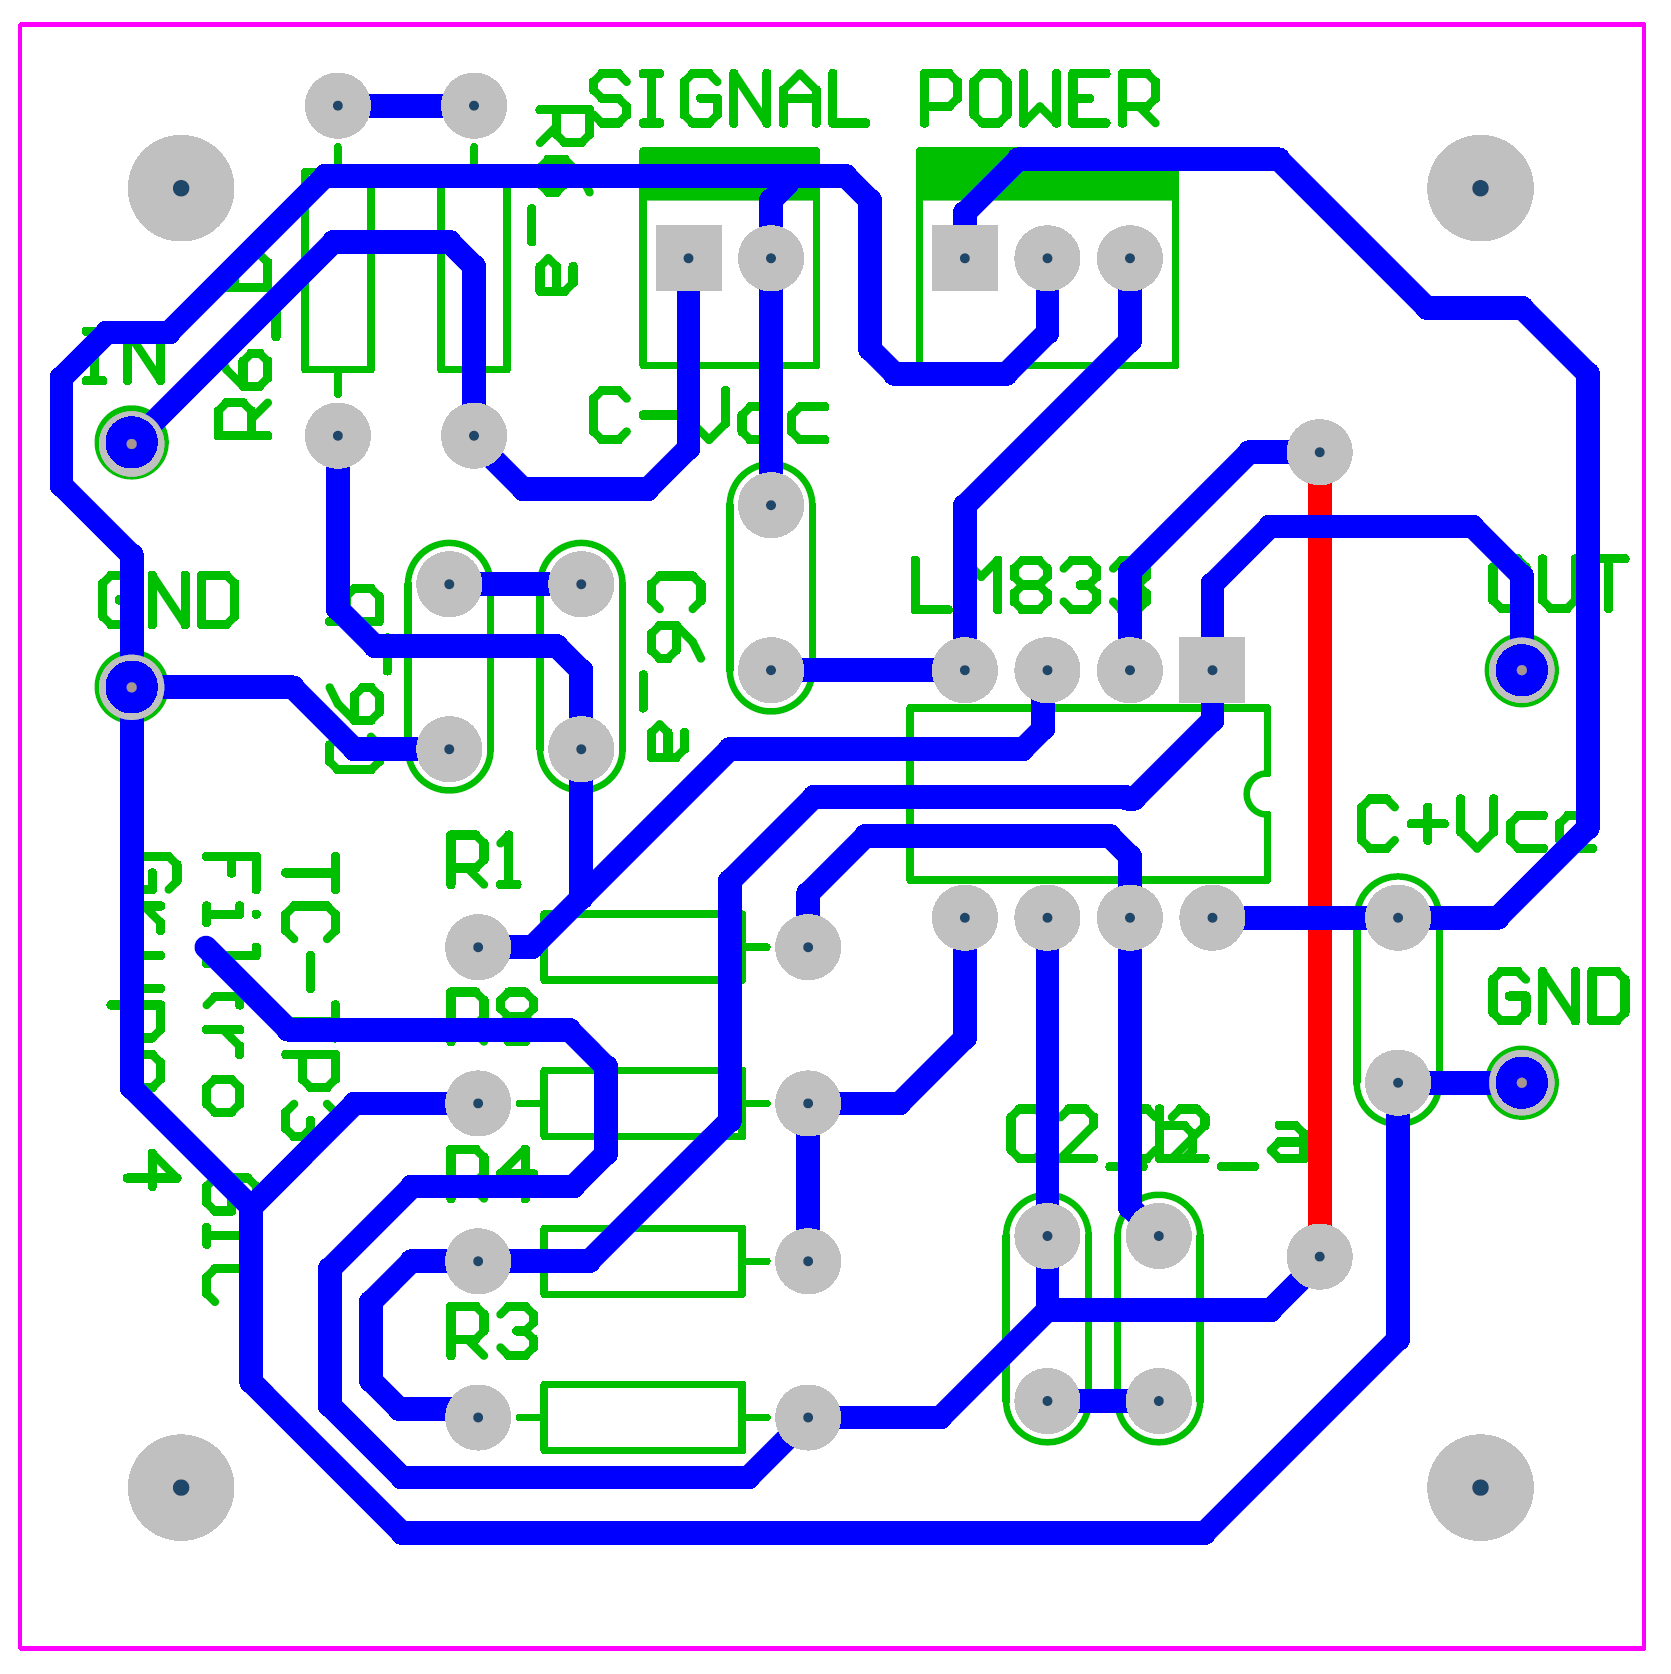
\includegraphics[scale=0.4]{../parte1/informe/resources/pcb}
\caption{Diseño final del circuito impreso}
\label{1_pcb}
\end{figure}

\section{Mediciones}
Se midieron las transferencias y la impedancia de entrada del circuito implementado, los resultados obtenidos me muestran a continuación, contrastados con los valores calculados y simulados.

\subsubsection{Transferencia}
La Figura \ref{1_bode} muestra las tres transferencias: calculada, simulada y medida. Se observa que el circuito implementado tiene una transferencia que se ajusta muy bien a la curva de transferencia deseada.

\begin{figure}[ht]
\centering
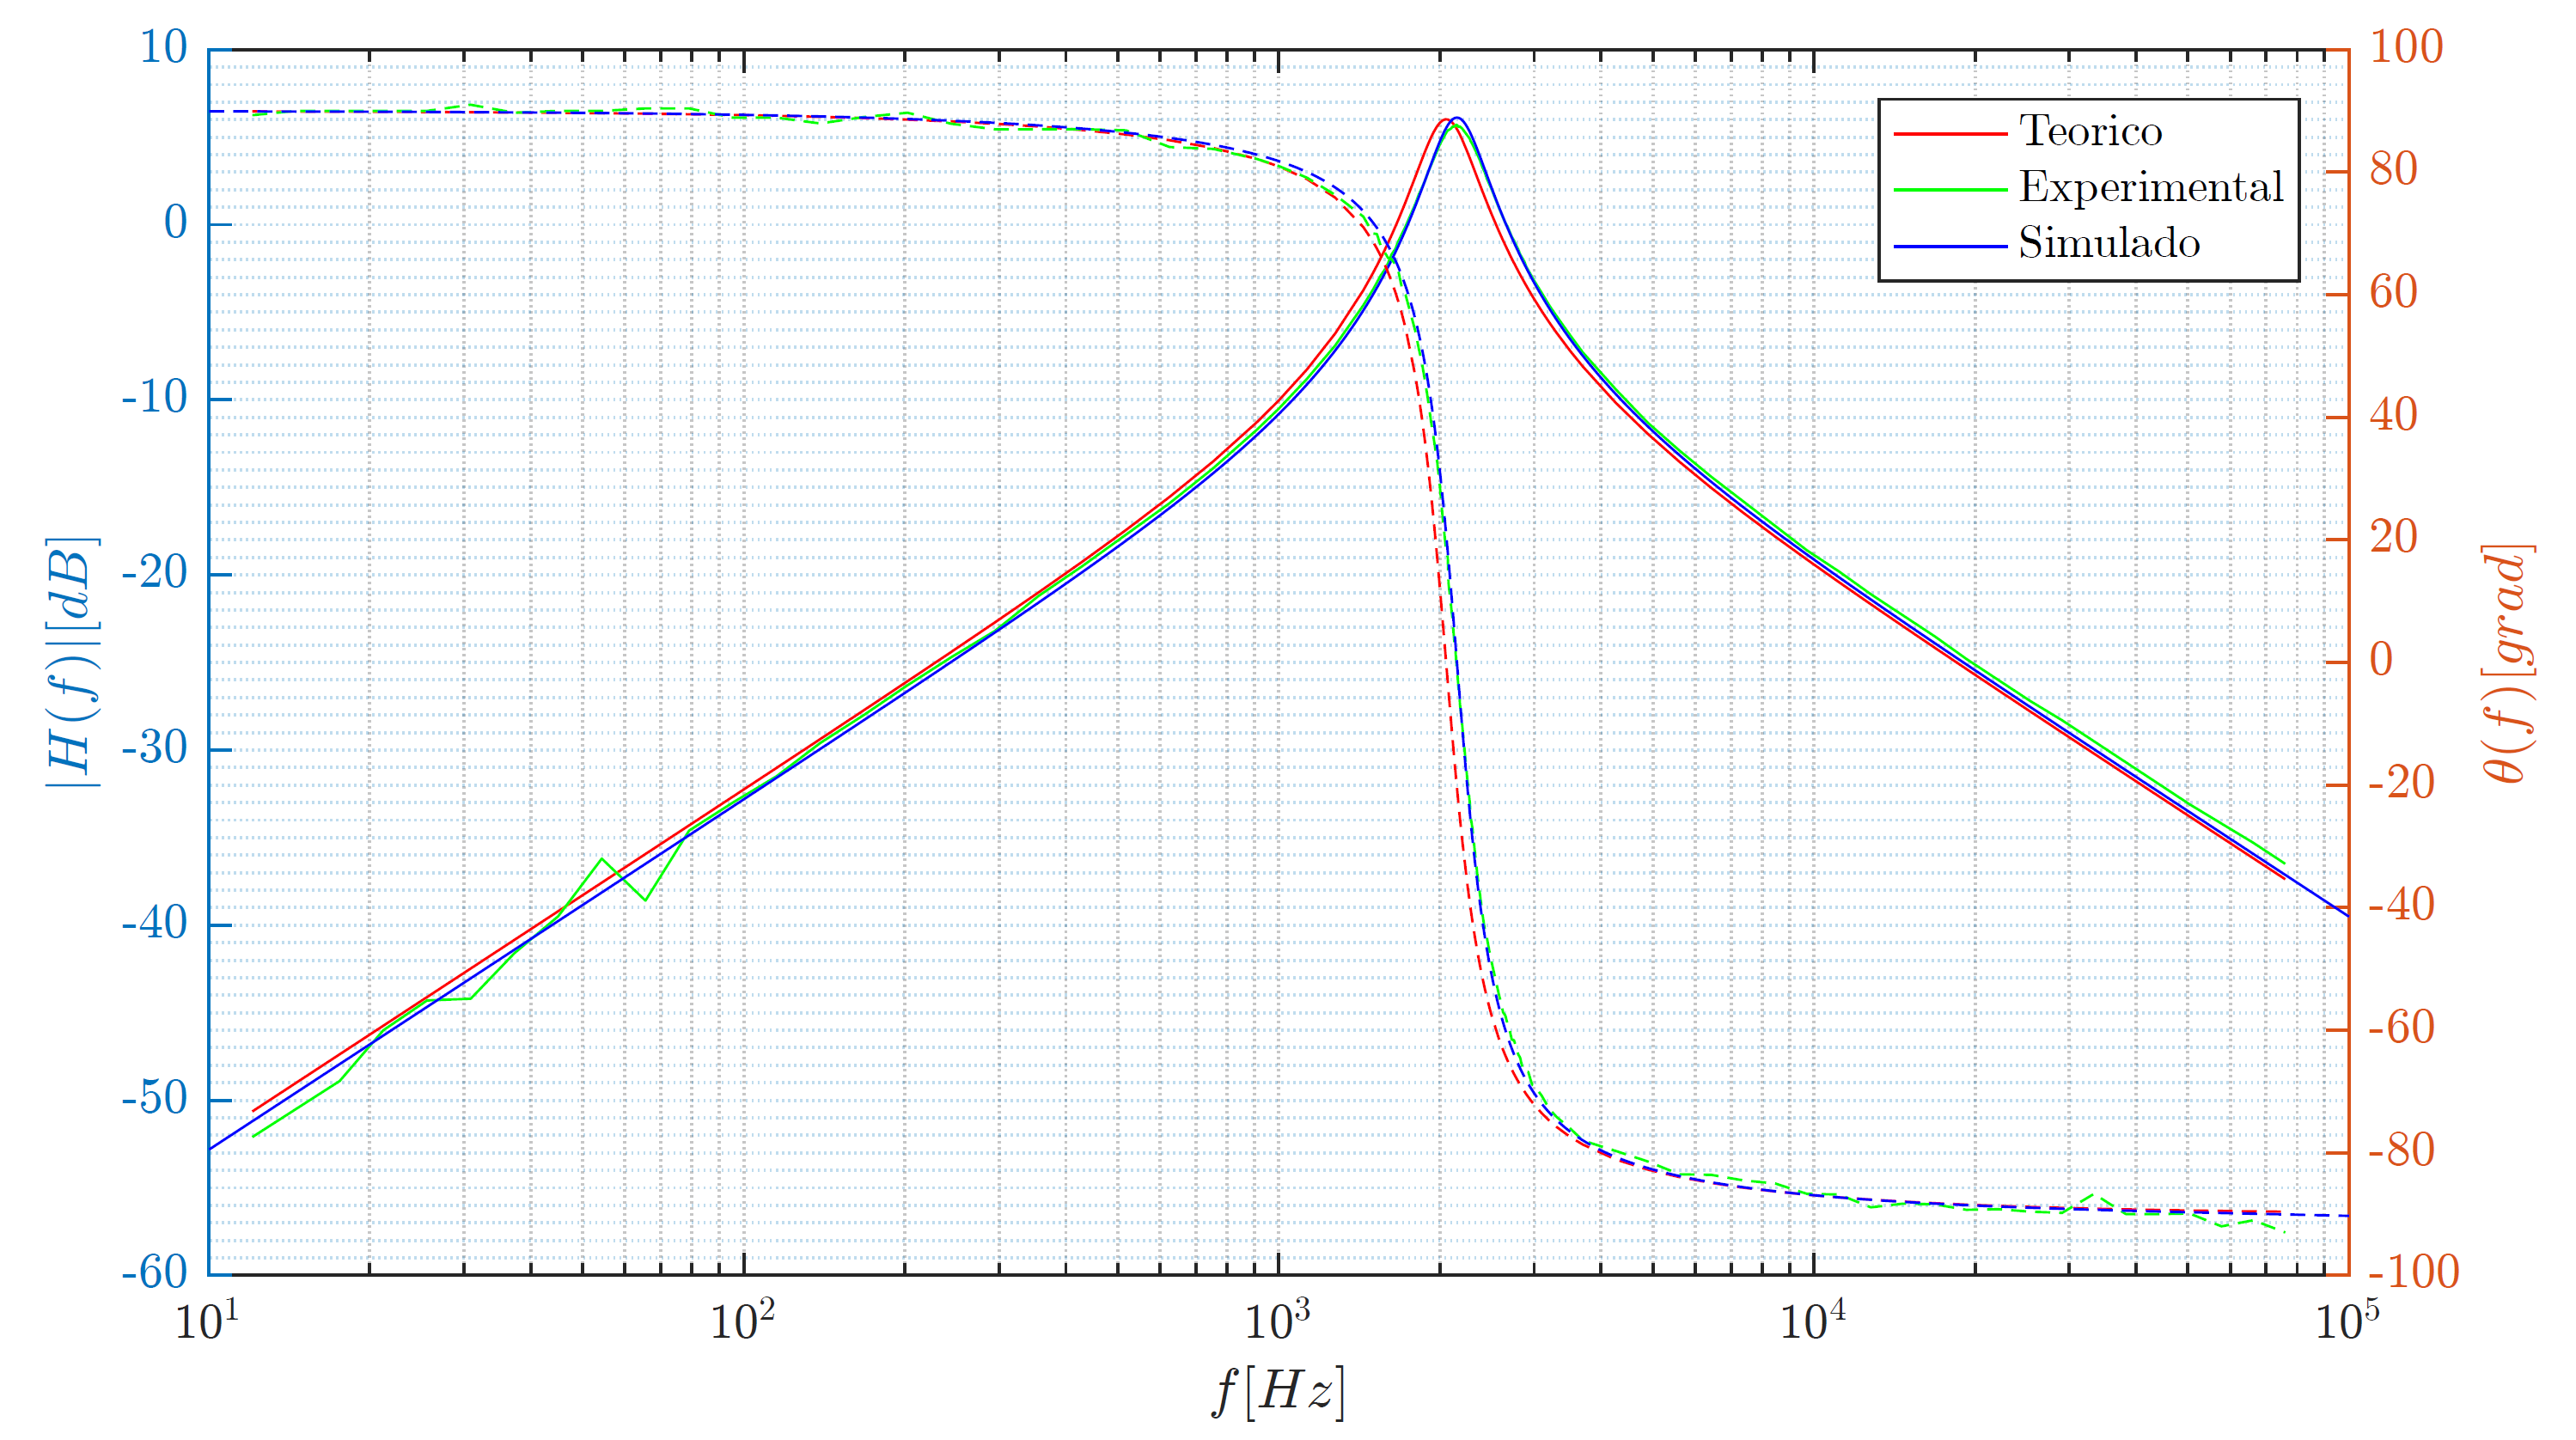
\includegraphics[scale=0.4]{../parte1/informe/resources/bode_todos}
\caption{Diseño final del circuito impreso}
\label{1_bode}
\end{figure}

\subsubsection{Impedancia de entrada}
Las figuras muestran la magnitud y la fase de la impedancia de entrada medida sobre el circuito implementado contra las calculadas. La impedancia de entrada calculada se muestra en la Expresión

\begin{figure}[H]
\centering
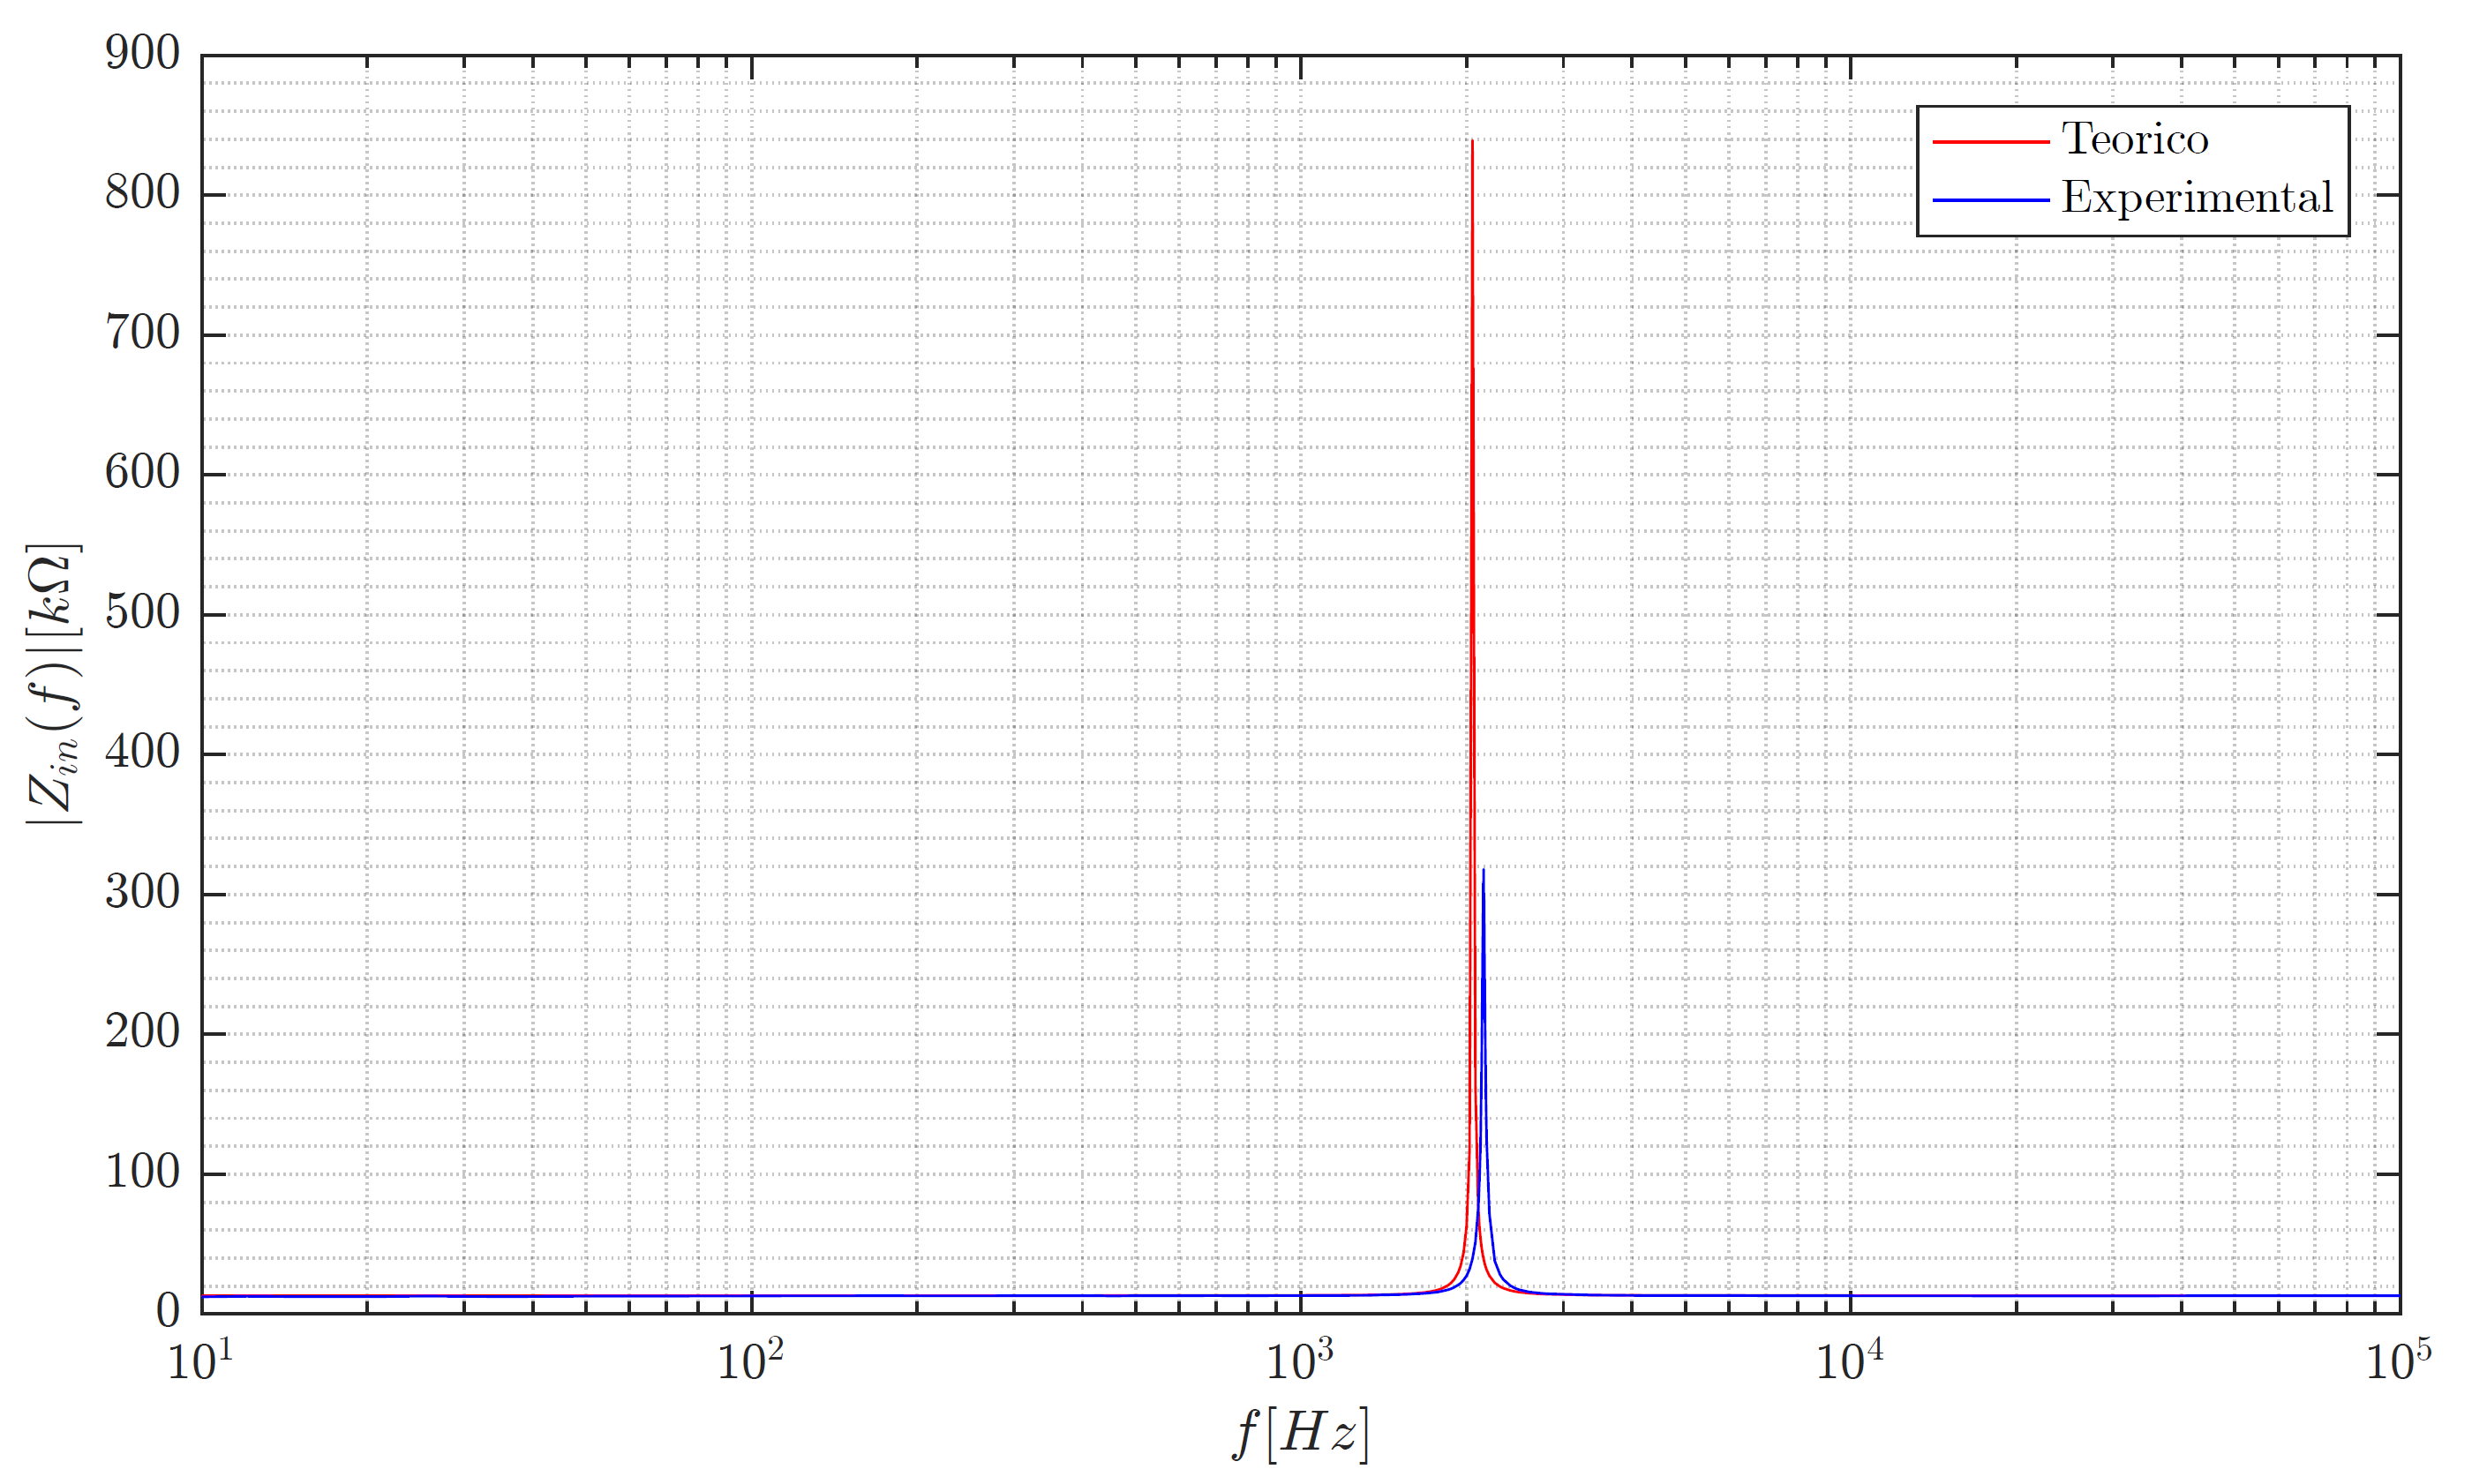
\includegraphics[scale=0.4]{../parte1/informe/resources/impedancia_entrada_mag}
\caption{Magnitud de impedancia de entrada medida vs. calculada}
\label{1_zin_mag}
\end{figure}

\begin{figure}[H]
\centering
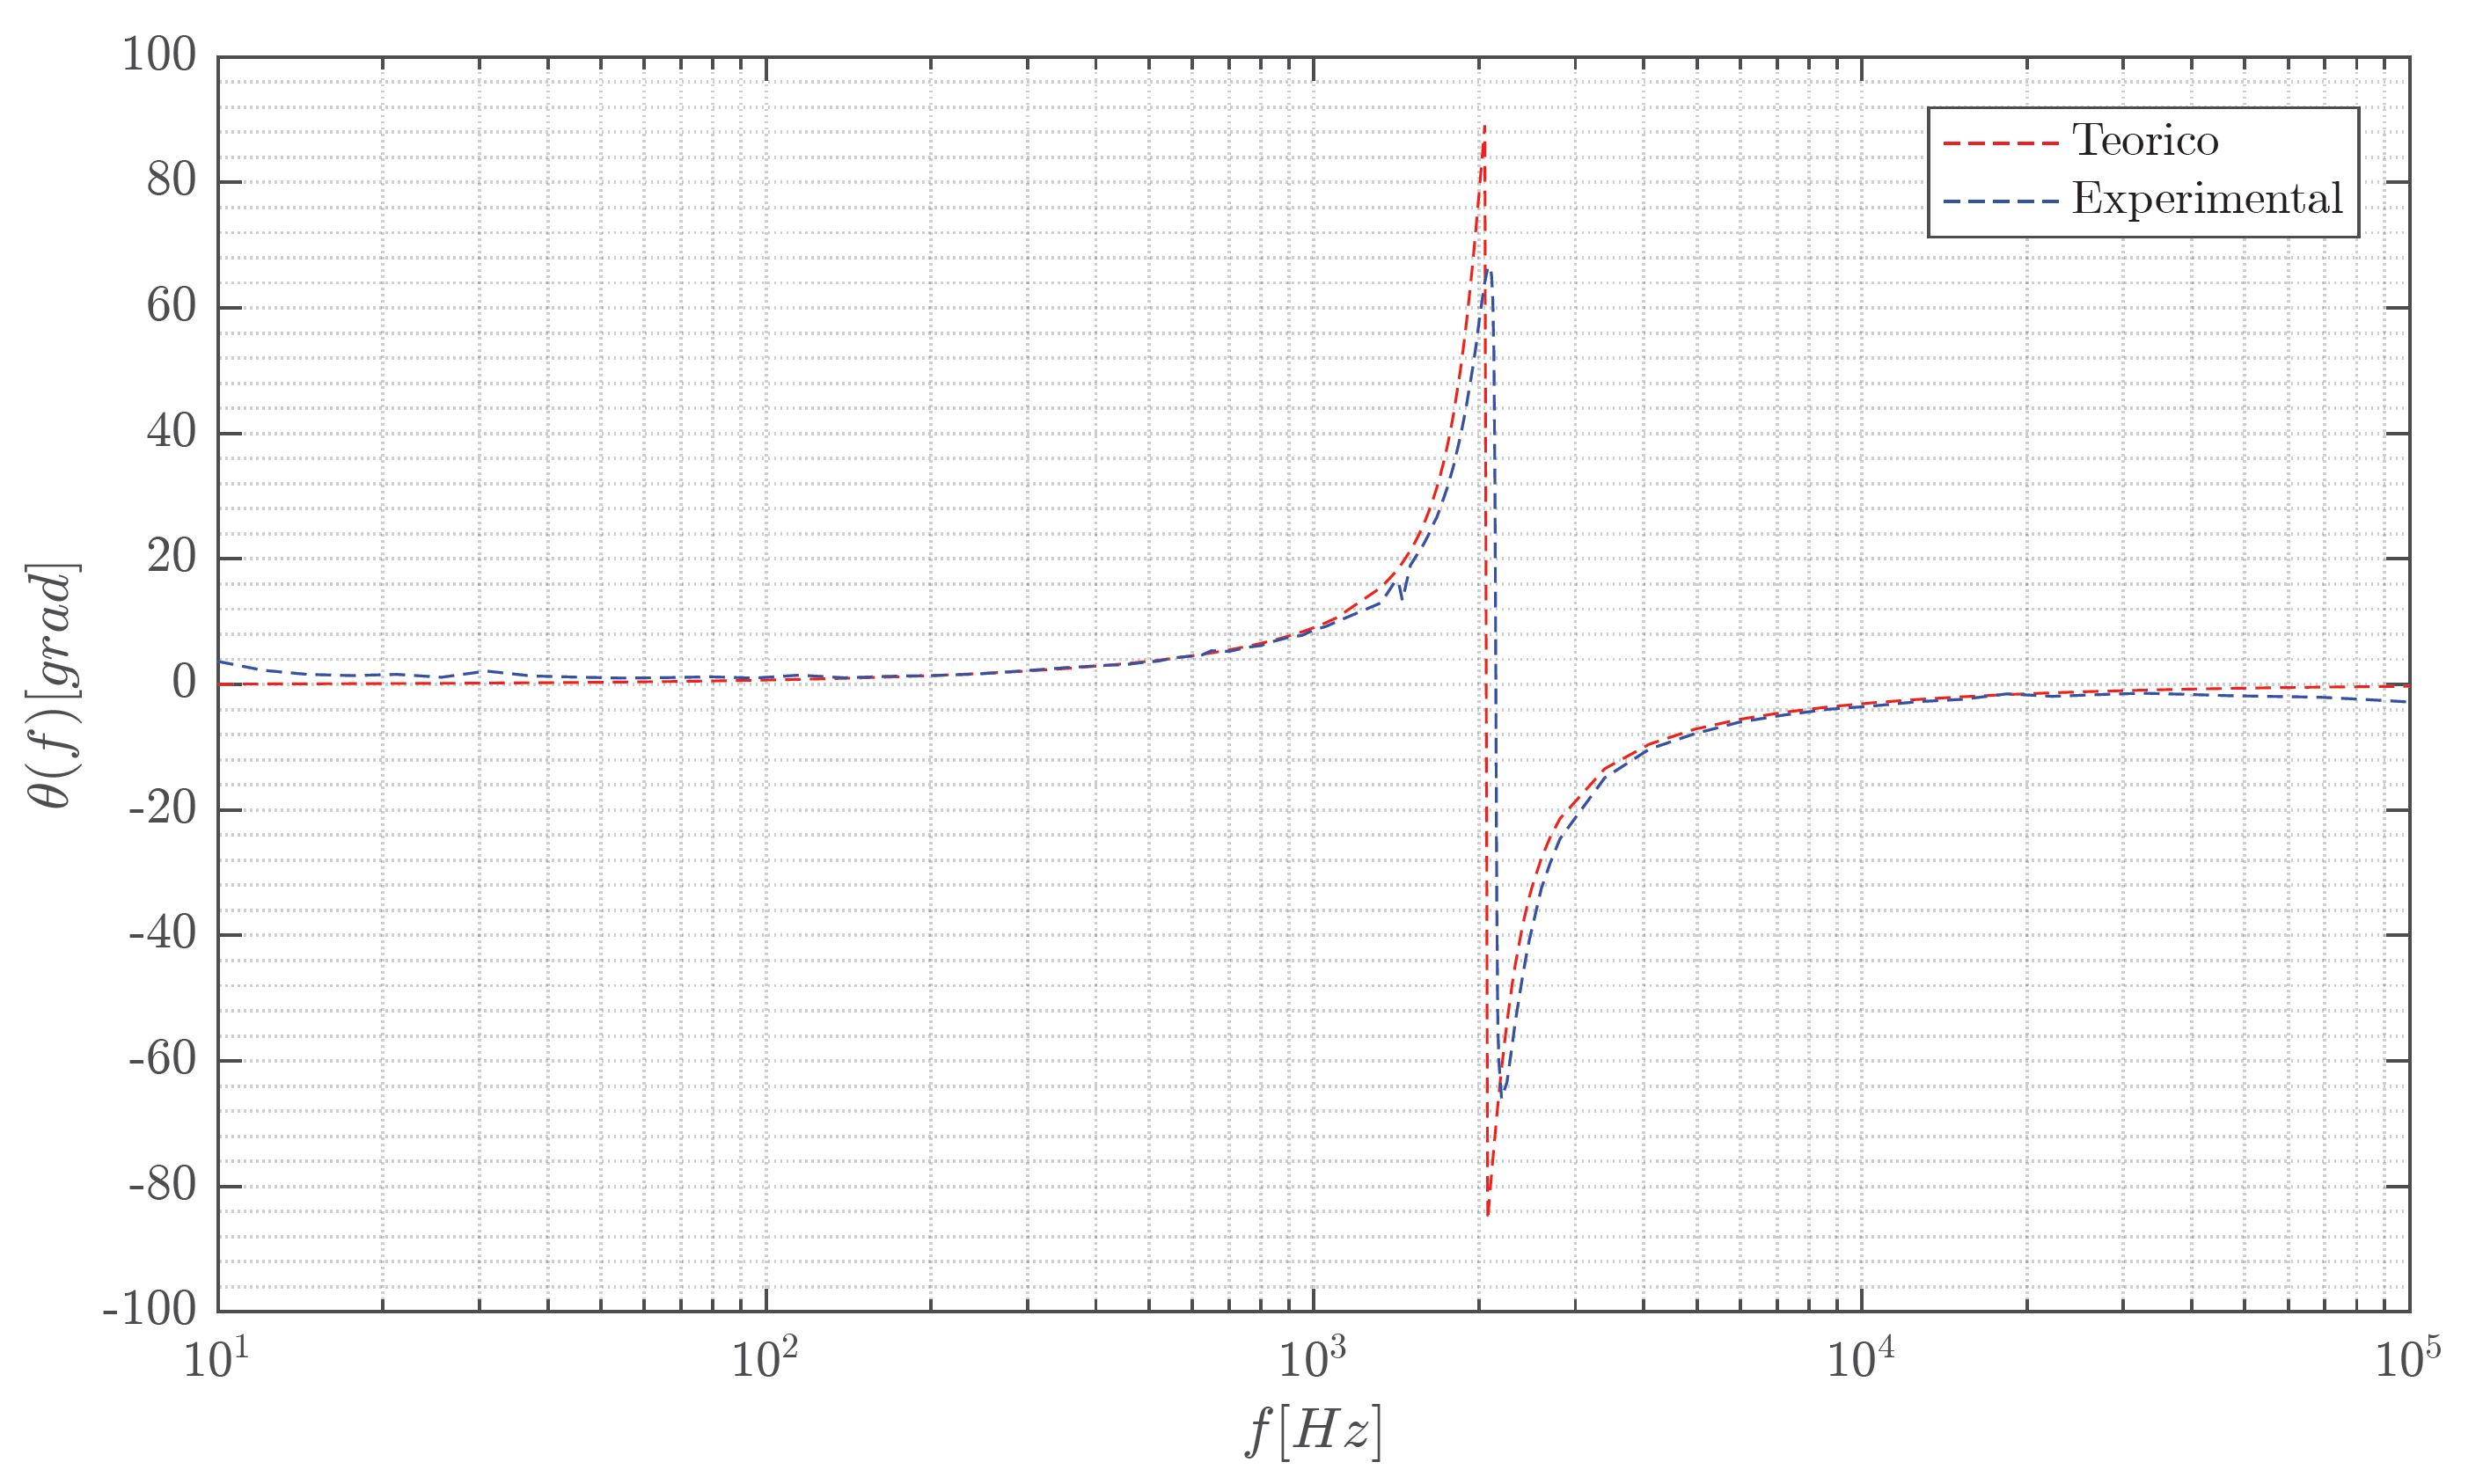
\includegraphics[scale=0.4]{../parte1/informe/resources/impedancia_entrada_phase}
\caption{Fase de impedancia de entrada medida vs. calculada}
\label{1_zin_phase}
\end{figure}

\begin{equation}
Z_{in}(\$) = \frac{R_6R^2C^2\$^2 + R^2C\$ + R6}{R^2C^2\$^2 + 1}
\label{1_zin_teo}
\end{equation}

\subsubsection{Error}

Las figuras \ref{1_mc_mag} y \ref{1_mc_phase} muestran los resultados obtenidos del análisis de Montecarlo realizado mediante la herramienta de simulación LTSpice. Para lograr observar las dispersiones se recortó el rango de frecuencias graficado entre 1kHz y 10kHz.

\begin{figure}[H]
\centering
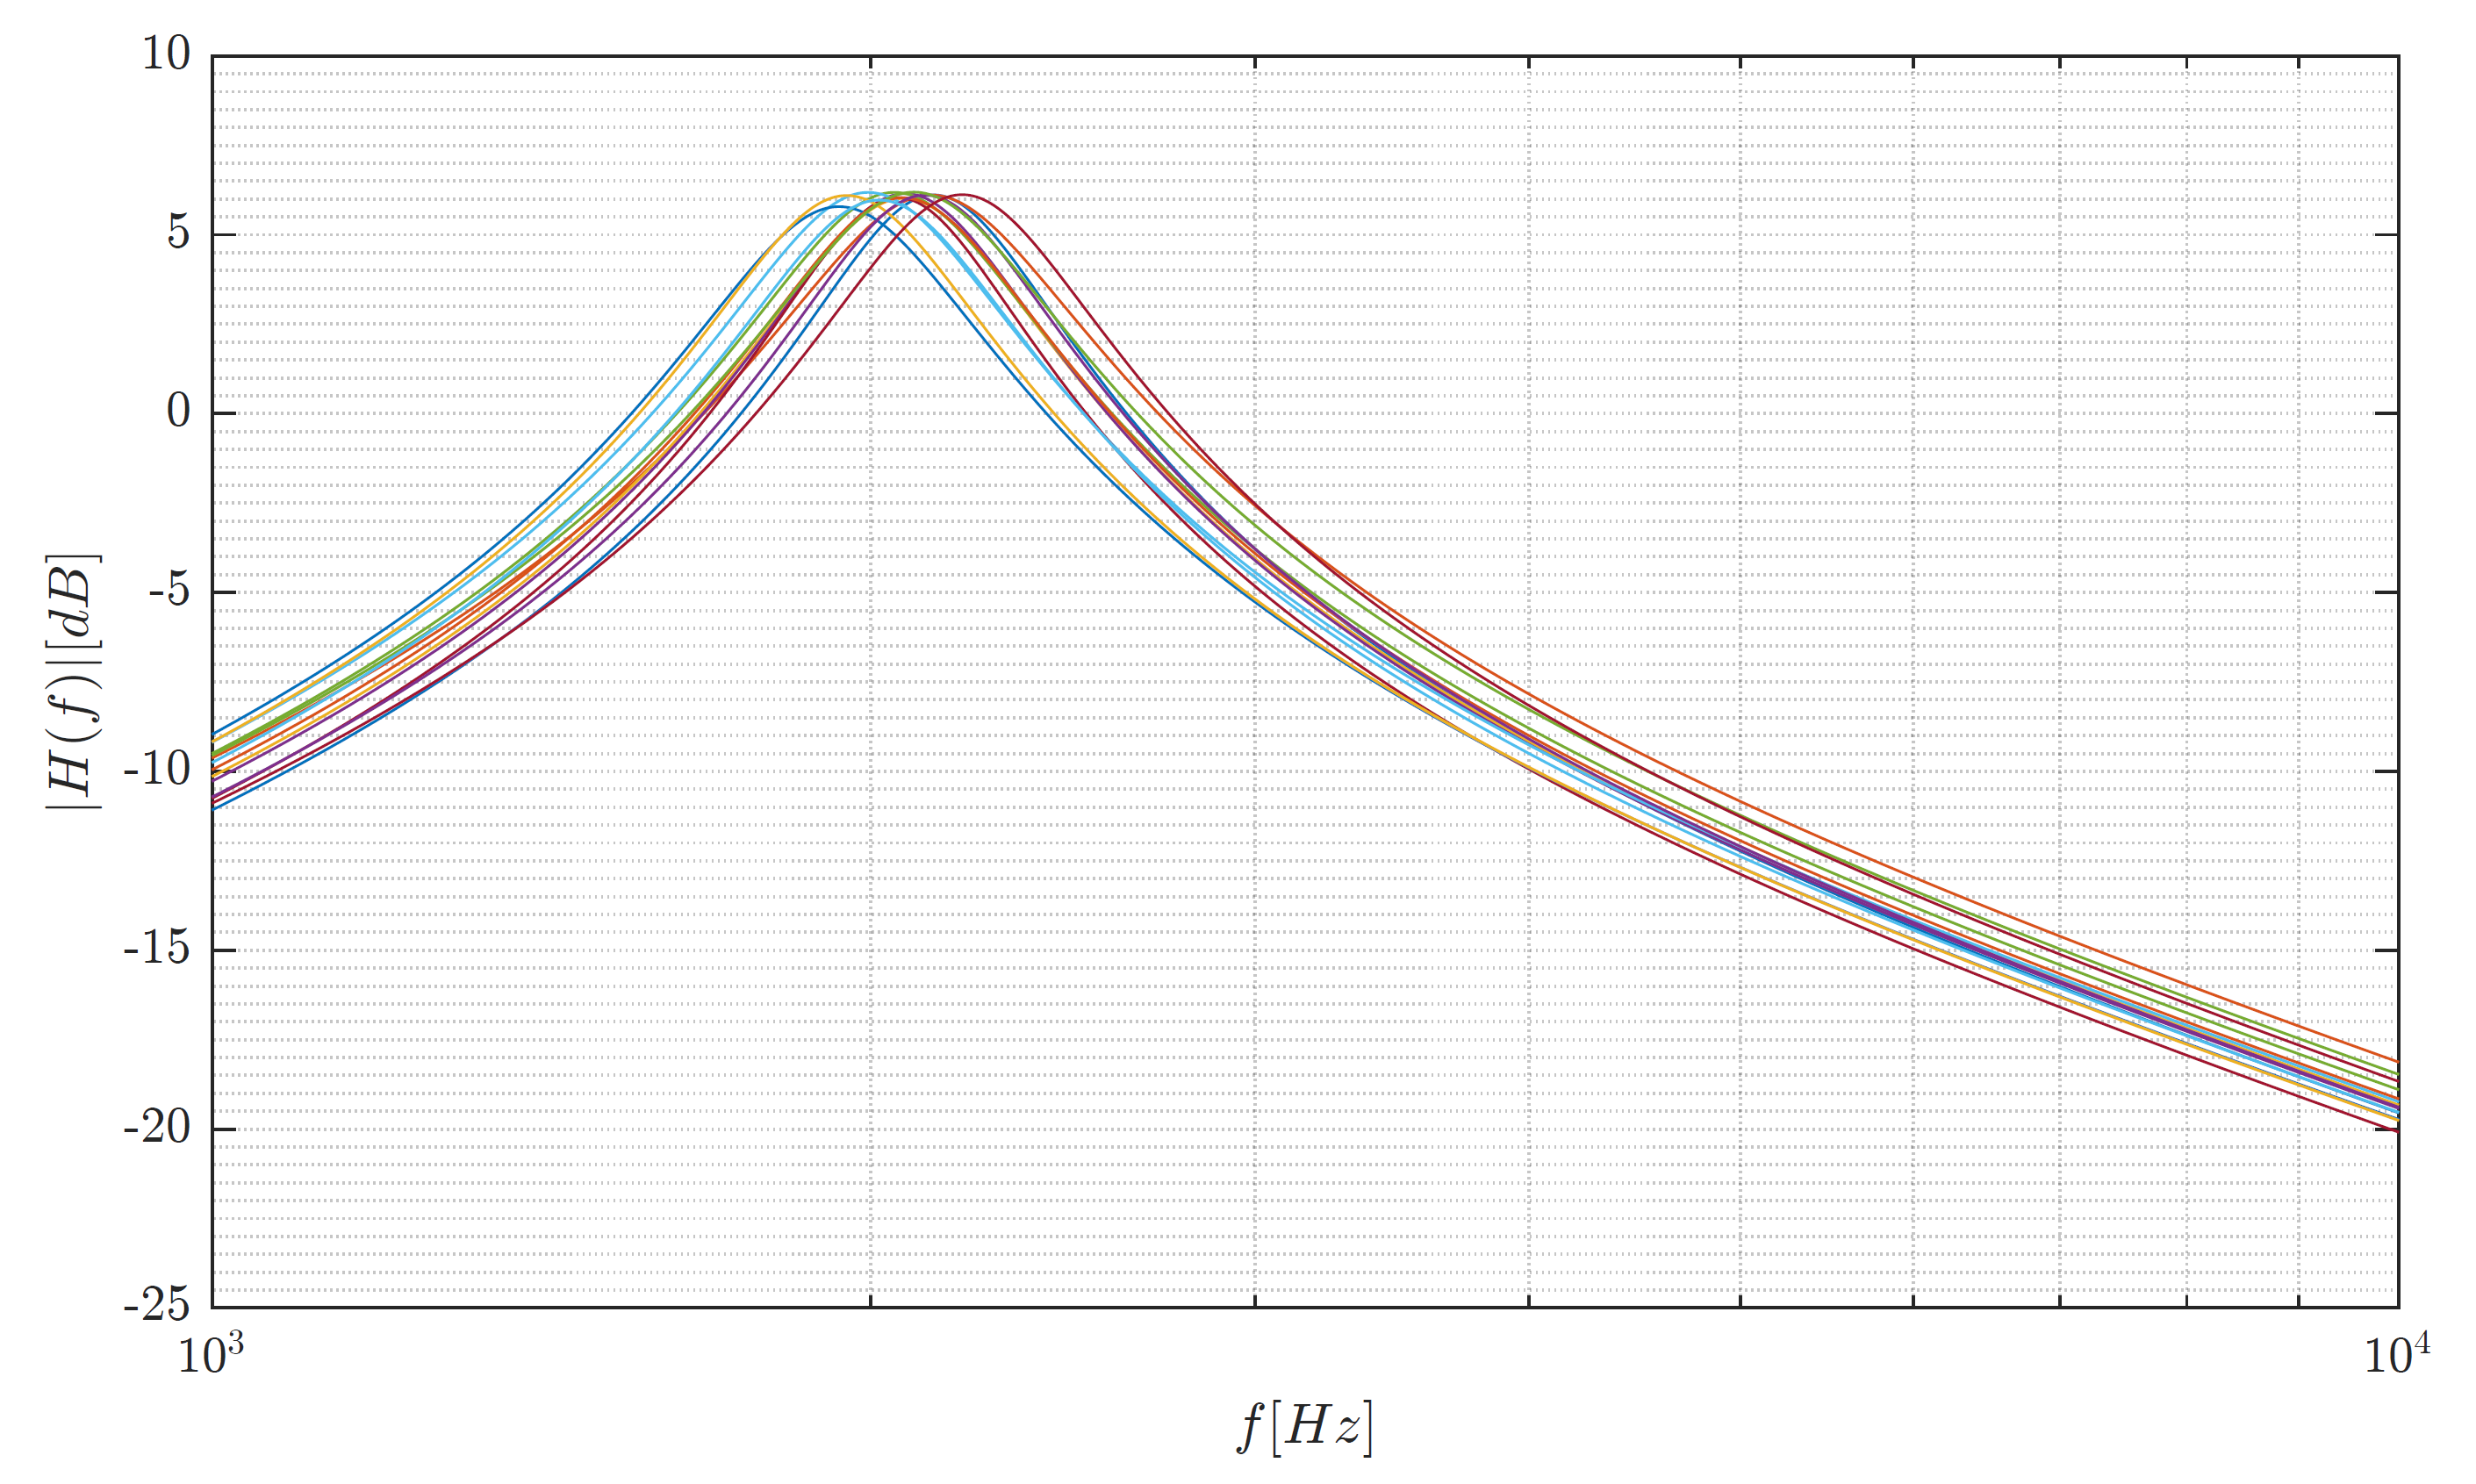
\includegraphics[scale=0.4]{../parte1/informe/resources/montecarlo_mag}
\caption{Análisis de Montecarlo. Transferencia en magnitud del circuito}
\label{1_mc_mag}
\end{figure}

\begin{figure}[H]
\centering
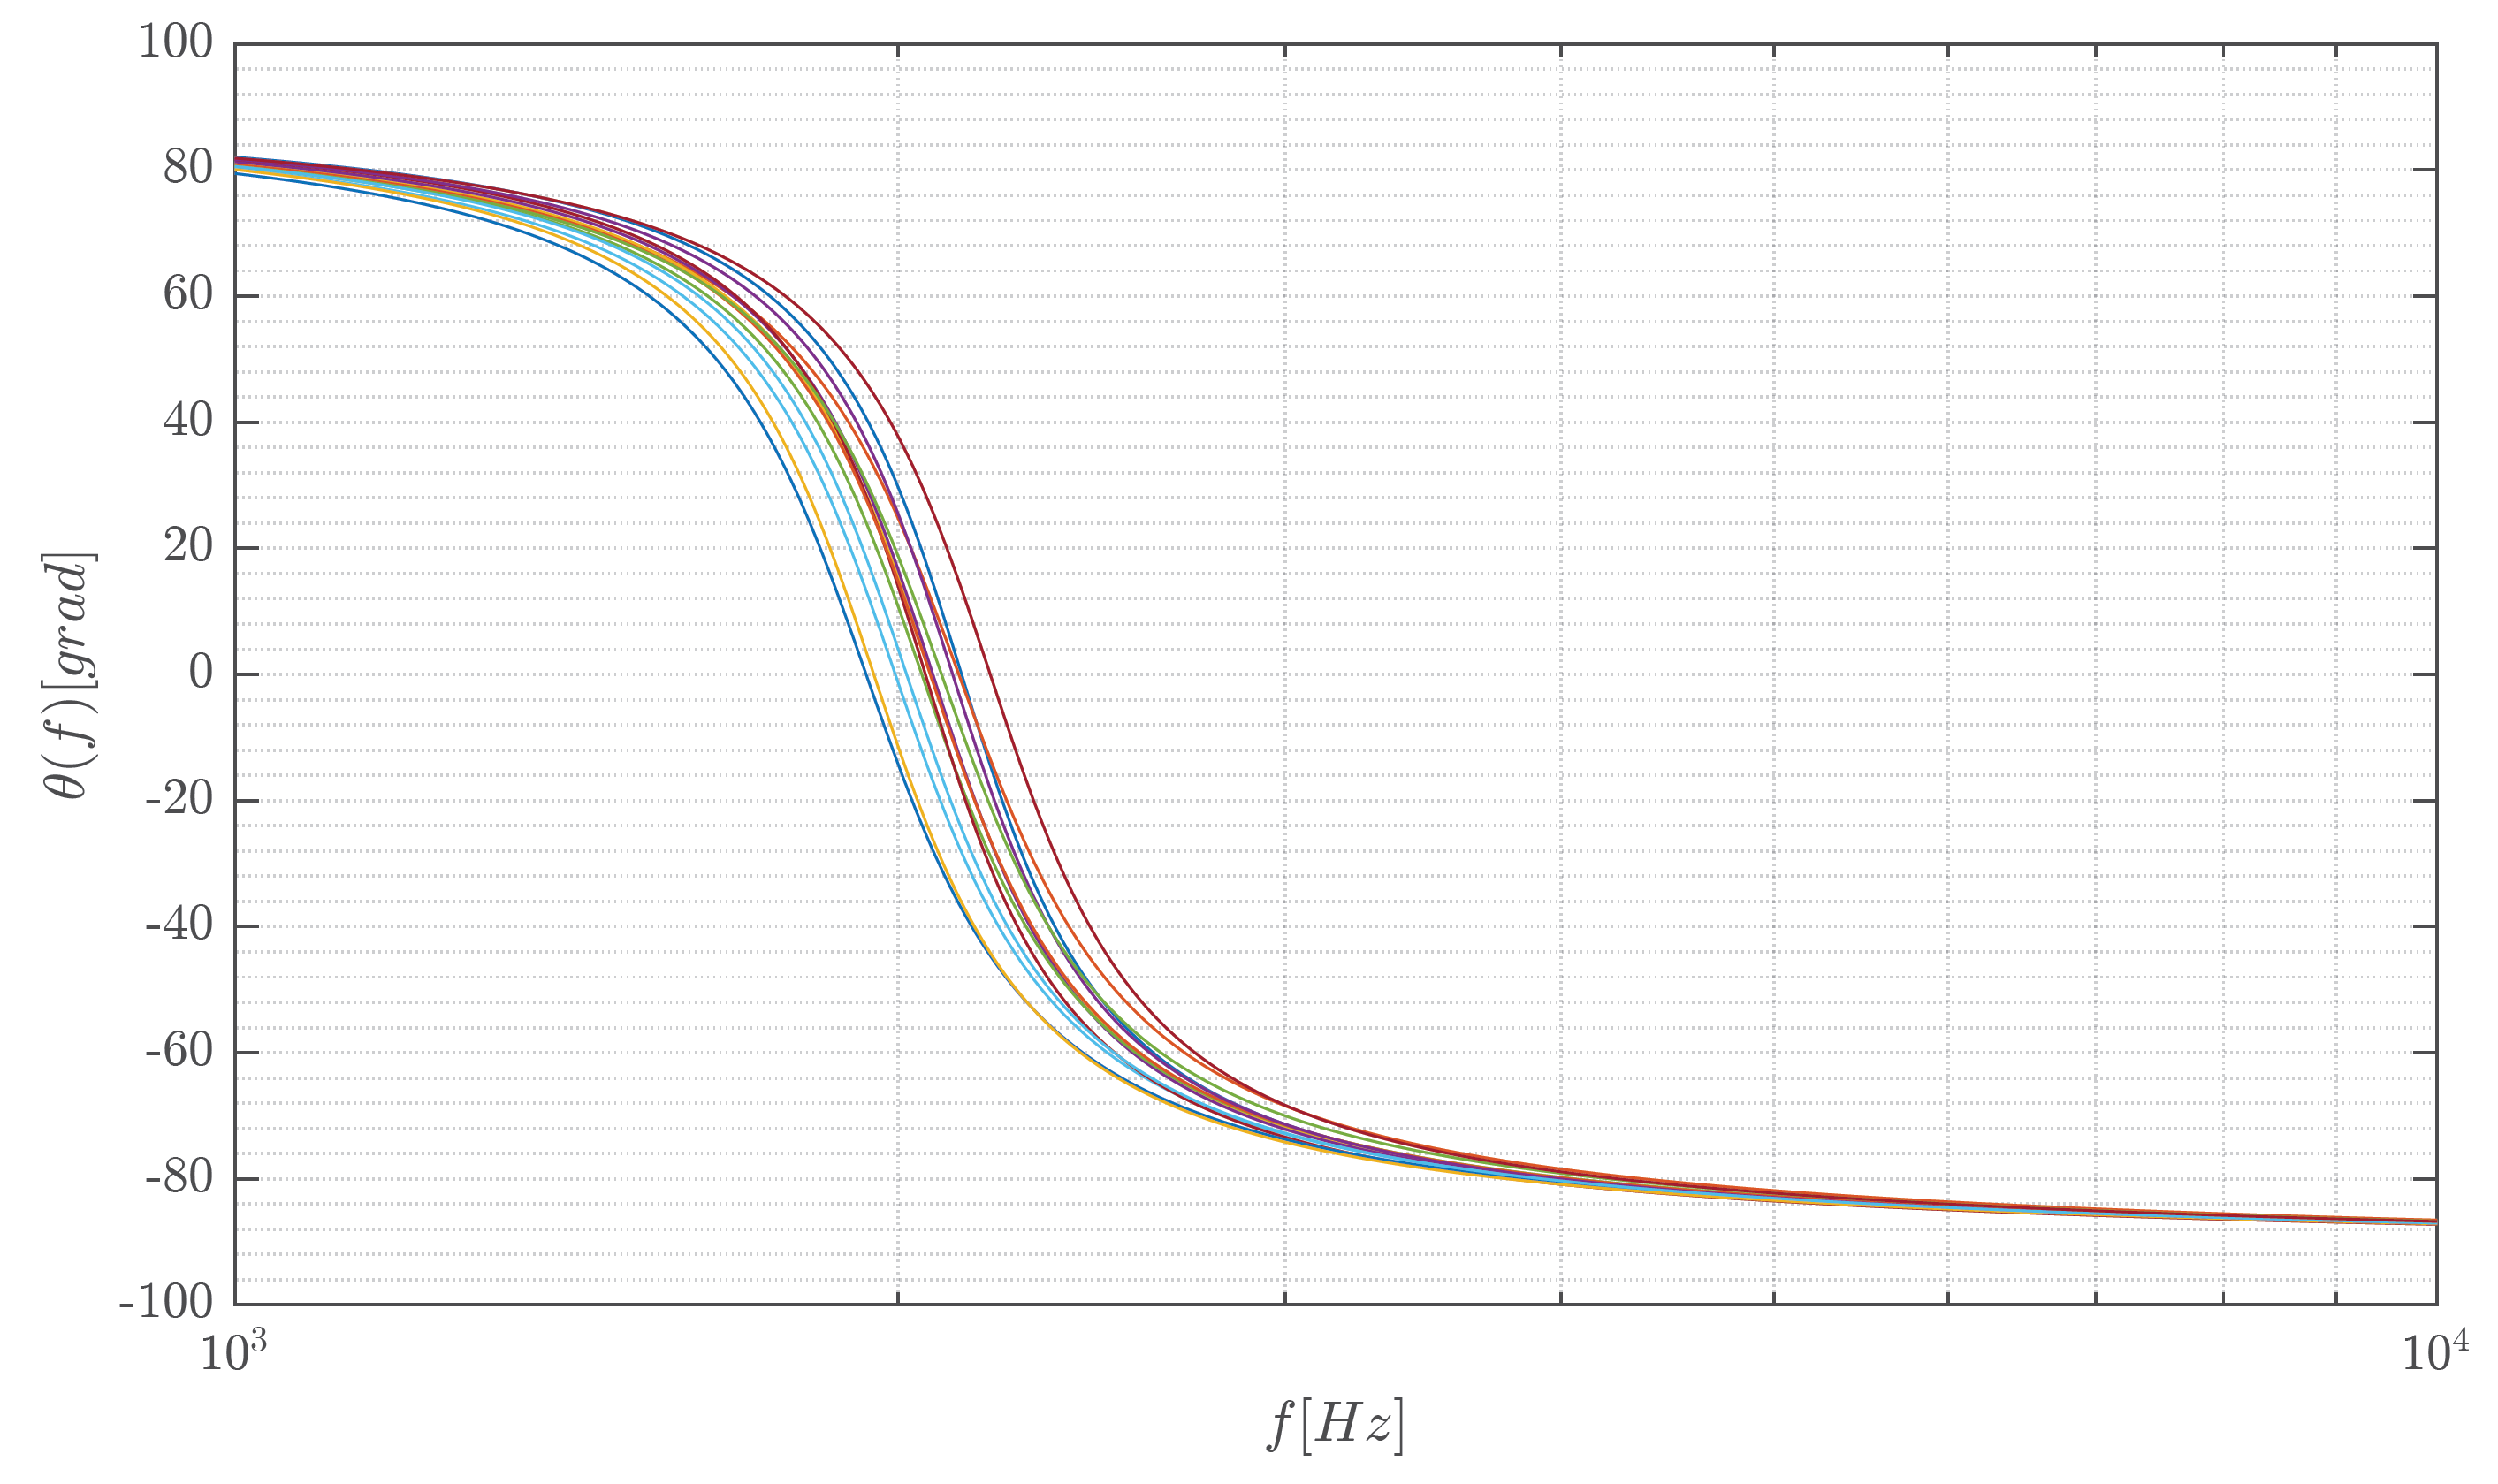
\includegraphics[scale=0.4]{../parte1/informe/resources/montecarlo_phase}
\caption{Análisis de Montecarlo. Transferencia de fase del circuito}
\label{1_mc_phase}
\end{figure}

El análisis se realizo imponiendo una tolerancia para los resistores del $5\%$ y del $10\%$ para los capacitores. En base a los datos arrojados por la simulación se realizó un cálculo de errores sobre la frecuencia central $f_0$. El máximo error absoluto calculado fue de $148.86Hz$, que representa un error porcentual del $7.25\%$


\section{Respuesta al escalón}
Se midió la respuesta al escalón del sistema, obteniéndose los resultados mostrados en la Figura \ref{1_step_response}. Las curvas correspondientes a la respuesta simulada y la respuesta teórica calculada se encuentran superpuestas, de forma tal que se dificulta observar la ínfima diferencia entre las curvas. Por otro lado, la curva de la respuesta al escalón medida, presenta una leve diferencia respecto a la respuesta teórica, aunque la misma se ajusta a la respuesta esperada.

\begin{figure}[H]
\centering
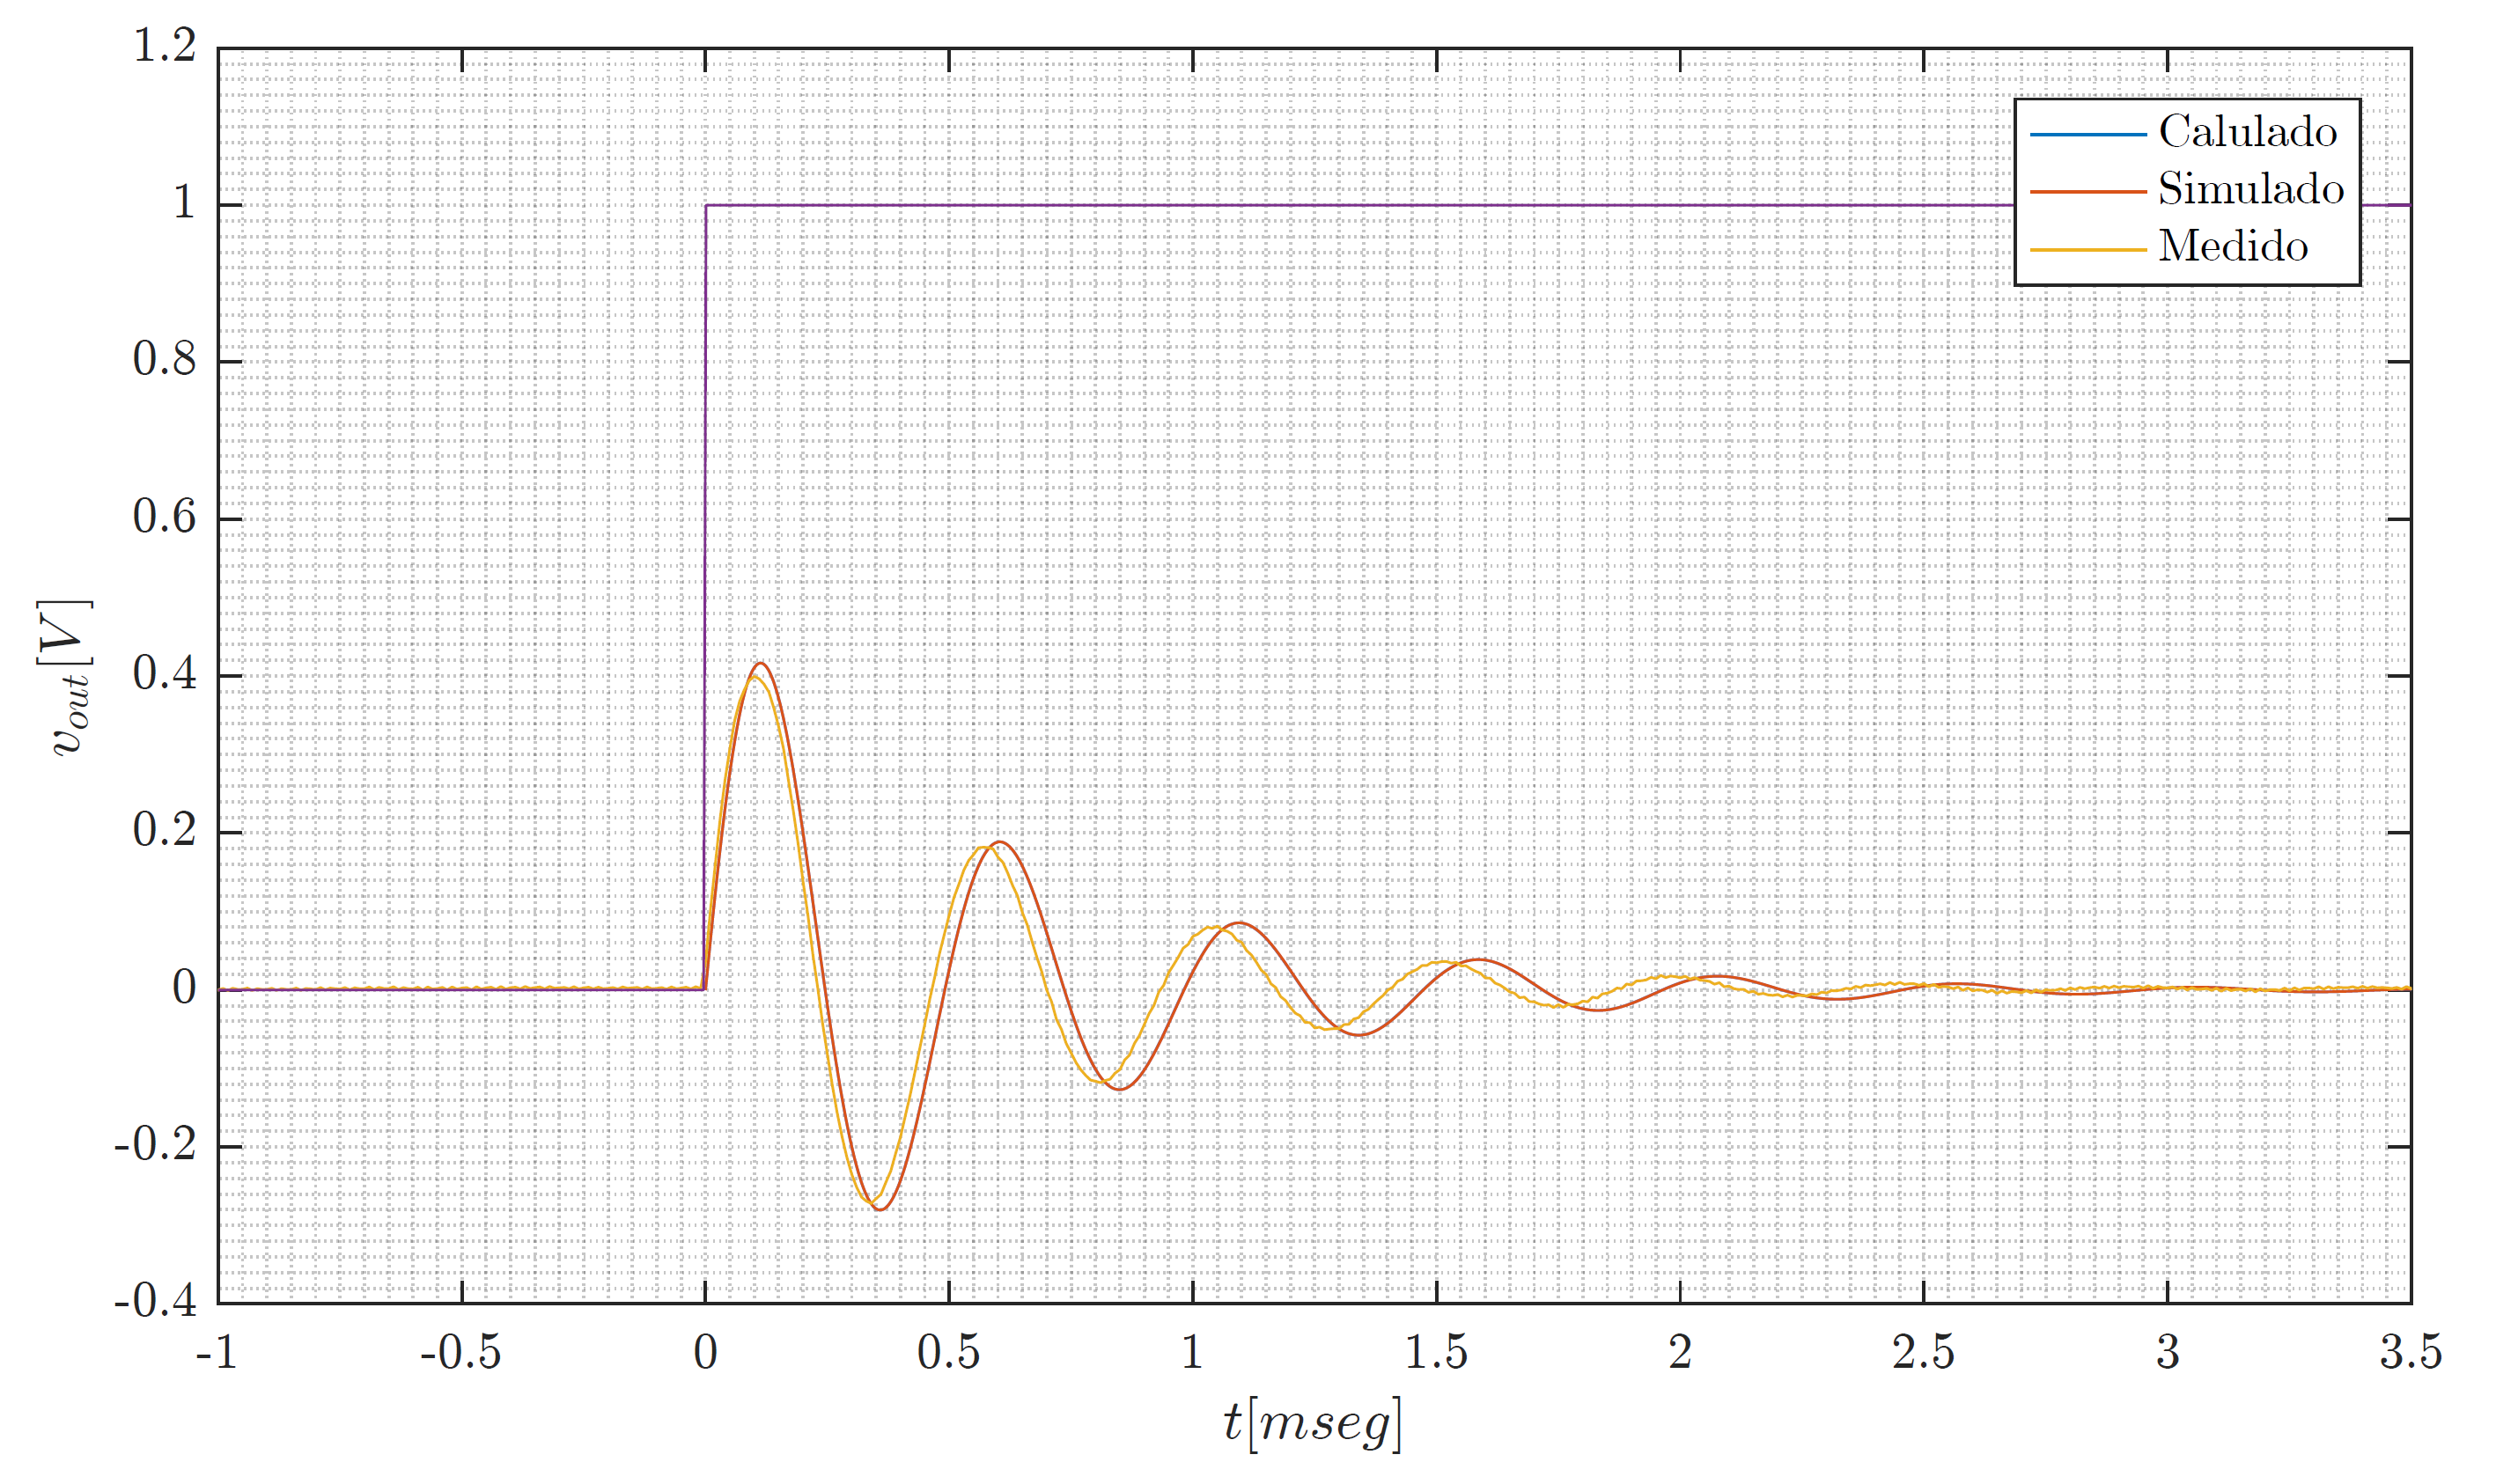
\includegraphics[scale=0.4]{../parte1/informe/resources/step_response}
\caption{Respuesta al escalón calculada, simulada y medida}
\label{1_step_response}
\end{figure}

La respuesta observada evidencia un sistema sub-amortiguado. Esto ya había quedado en evidencia en la caracterización de los polos de la transferencia del circuito, en la sección \ref{1_seccion_r6}

\section{Conclusiones}
Del análisis realizado sobre el circuito presentado en el desarrollo del informe, se pueden concluir dos ítem destacables. En primer lugar se destaca la precisión con la que los datos exprerimentales se ajustan a los cálculos realizados.
Por otro lado, y como principal objeto del informe, se debe destacar la buena aproximación a una inductancia 'real' que proporciona el circuito GIC. 